
%%\input boostsymbols.tex

%%\authorrunning{G. Soyez, A. Schwartzman (ed.) et al.} 
{\it Section prepared by the Working Group: 'Jet substructure performance at high luminosity', P. Loch, D. Miller, K. Mishra,  P. Nef, \underline{A. Schwartzman}, \underline{G. Soyez}.
}

%\title{Study of grooming performance in the presence of large pile-up at the LHC}

%\author[1]{P.~Loch}
%\author[2]{D.~Miller}
%\author[4]{K.~Mishra}
%\author[3]{P.~Nef}
%\author[3]{A.~Schwartzman}
%\author[5]{G.~Soyez}

%\affil[1]{Department of Physics,	University of Arizona, Tucson, Arizona 85721, USA}
%\affil[2]{Enrico Fermi Institute, University of Chicago, Chicago, Illinois 60673, USA}
%\affil[3]{SLAC, Menlo Park, Callifornia 94025, USA}
%\affil[4]{Fermilab, Batavia, Illinois 60510, USA}
%\affil[5]{IPhT CEA Saclay, F-91191 Gif-sur-Yvette Cedex, France}  

%\maketitle


%%\subsection{Monte Carlo evaluations of pile-up jet production in minimum bias proton-proton collisions at \cms{} energies \sqrts{8}}

The first LHC analyses exploring the experimental response to jet substructure
demonstrated that the highly granular ATLAS and CMS detectors can yield 
excellent performance. They also confirmed the susceptibility of 
the invariant mass of large-area jets to the energy flow from the 
additional proton-proton interactions that occur each bunch crossing. 
And, finally, they provided a first hint that jet grooming could be a 
powerful tool to mitigate the impact of pile-up. Since then, the LHC
collaborations have gained extensive experience in techniques 
to correct for the impact of pile-up on jets. In this Section 
these tools are deployed in an extreme pile-up environment. 
We simulate \pu{} levels as high as $\axing = 200$, such as may be
expected in a future high-luminosity phase of the LHC. We evaluate
the impact on jet reconstruction, with a focus on the (substructure) 
performance.


%\subsection{Introduction} \label{subsec:intro}
\subsection{Pile-up}
Each LHC bunch crossing gives rise to a number of \pp{} collisions and typically the hard scattering (signal) interaction is accompanied by several additional \pu{} \pp{} collisions. The total \pp{} cross-section is about $\sigma_{\mathrm{tot}} = 98$ mb (inelastic $\sigma_{\mathrm{inel}} = 72.9$ mb) at \sqrts{7} \cite{Antchev:2013iaa}, and even slightly higher at \sqrts{8}{} in 2012. With a peak instantaneous luminosity of about $7.7 \times 10^{33}$~cm$^{-2}$~s$^{-1}$ in 2012, the resulting average number of \pu{} collisions reached $\axing = 20$ at the highest intensities. The 2012 data set has a rather flat $\mu$ distribution extending from $\mu = 5$ to $\mu = 35$. In future \LHC{} running even higher \axing{} are expected. 

\PU{} manifests itself mostly in additional hadronic transverse momentum 
flow, which is generated by overlaid and statistically independent, 
predominantly soft \pp{} collisions that we refer to as 
``minimum bias'' (MB). This diffuse 
transverse energy emission interferes with the signal of hard scattering 
final state objects like particles and particle jets, and typically 
requires corrections, in particular for particle jets.  In addition,
 it can generate particle jets (\emph{\pujet s}) either from any of 
the individual \MB{} collisions (\emph{\qcdjet s}), or by stochastically 
forming jets in the high density particle flow generated by the 
multitude of them (\emph{\stojet s}).  
%, which occupy a larger area in the event rapidity-azimuth plane.


\subsection{Monte Carlo event generation} \label{subsec:mc} 

We model the \pu{} with \MB{} collisions at \sqrts{8} and
a bunch spacing of 50 ns, generated with the \pythia{} Monte Carlo
(MC) generator~\cite{pythia,pythia8}, with its 
{\sc 4C} tune  \cite{Corke:2010yf}. 
All inelastic, single diffractive, and double diffractive processes are 
included, with the default fractions as provided by \pythia (tune 4C). 
%Fig.~\ref{fig:interaction} summarizes some of the features of the 
%particle flow in these single collision events. 

Overall $100\times 10^{6}$ \MB{} events are available for 
pile-up simulation. The corresponding data are generated in samples of 
$25000$ \MB{} collisions, with the largest possibly statistical 
independence between samples, including new random seeds for each sample. 
To model pile-up for each signal interaction, the stable 
particles\footnote{A particle is considered stable if its lifetime $\tau$ 
in the laboratory frame of reference passes $c\tau > 10$~mm.} generated 
in a number $\mu$ of \MB{} collisions, with $\mu$ being sampled from a 
Poisson distribution around the chosen \axing, are added to the final 
state stable particles from the signal. This is done dynamically by an 
event builder in the analysis software, and is thus not part of the 
signal or \MB{} event production. All analysis is then performed on 
the merged list of stable particles to model one full collision event 
at the \LHC. 

%\begin{figure*}[htbp!]\centering
%\subfigure[Particle number density in individual \MB{} interations]{\includegraphics[angle=90,width=0.46\textwidth]{figures/npart_vs_rap}\label{fig:interaction:nvert}}
%\subfigure[Particle \pT{} flow]{\includegraphics[angle=90,width=0.46\textwidth]{figures/pt_flow}\label{fig:interaction:ptvert}}
%\caption[]{The number of particles per unit area in rapidity and azimuth $\partial N^{2}/(\partial \rap \partial \azi)$ is shown in \subref{fig:interaction:nvert}, as function of the particle rapidity $y$. The transverse momentum generated by these particles is shown in \subref{fig:interaction:ptvert}, both as an average per particle ($\langle \pT \rangle(\rap)$, blue) and summed in bins of $y$ ($\langle \Sigma \pT\rangle (\rap)$, red). The stable particle final state from \pythia{} is used to generate the shown features.}
%\label{fig:interaction}
%\end{figure*}


The example signal chosen for the Monte Carlo simulation based studies
presented in this Section is the decay of a possible heavy \Zprime{}
boson with a chosen $\ZprimeM = 1.5$~\tev{} to a (boosted) top
quark pair, at \sqrts{8}. The top- and anti-top-quarks then decay 
fully hadronically ($t \to \Wboson b \to jj\,\bjet$) or 
semi-leptonically ($t \to \Wboson b \to \ell \nu\,\bjet$). 
The \pythia{} generator \cite{pythia,pythia8} is used to generate the 
signal samples. The soft physics modeling parameters in both cases are 
from the pre-LHC-data tune 4C  \cite{Corke:2010yf}.  
The pile-up is simulated by overlaying generated minimum bias
\pp{} interactions at \sqrts{8} using Poisson distributions with
averages $\axing = \{ 30, 60, 100, 200 \}$, respectively, thus
focusing on the exploration of future high intensity scenarios at
\LHC.



All analysis utilizes the tools available in the \FJ{} \cite{Cacciari:2011ma} 
package for jet finding and jet sub-structure analysis. The larger jets used 
to analyze the final state are reconstructed with the \antikt{} 
algorithm~\cite{Cacciari:2008gp} with  $R = 1.0$, to assure that most of 
the final state top-quark decays can be collected into one jet. This 
corresponds to top-quarks generated with $\pT \gtrsim 400$~\GeV. 
The configurations for jet grooming are discussed 
in Section \ref{sec:grooming}. 




\subsection{Investigating jets from \pu} \label{sec:investigation}

Stable particles emerging from the simulated \pp{} collisions are clustered into \antikt{} jets \cite{Cacciari:2008gp} with
a radial distance parameter $R=0.4$, using the \FJ{} \cite{Cacciari:2011ma} implementation:
\begin{description}
    \item{\bf Truth jets} are obtained by clustering all stable particles from a given individual \MB{} interactions. For an event containing
        $\mu$ pileup interactions, jet finding is therefore executed $\mu$ times.
	The resulting truth jets are required to have $\pT \geq 5$~\GeV. 
    \item{\bf Pileup jets} are obtained by clustering the stable particles from all \MB{} 
            interactions forming the \pu{} event. They are subjected to the kinematic cuts described below. 
\end{description}
Jets with rapidity $|y|<2$ are accepted.

The contribution of \pu{} to jets can be corrected using the jet area based method in Ref.~\cite{Cacciari:2007fd}. It employs the median transverse momentum density $\rho$, which here is determined using \kT{} jets with $R = 0.4$ within $|y| < 2$.   To evaluate the effect of this correction, the transverse momentum ratio \Rpt{} is introduced as
\begin{equation}
\Rpt =\dfrac{\ptmatch}{\pT - \rho A} = \dfrac{\ptmatch}{\ptcorr}.
\label{eq:match}
\end{equation} 
Here $A$ is the catchment area \cite{Cacciari:2008gn} of the \pujet, and \ptmatch{} is the matching truth jet \pT. The matching criterion is similar to the one suggested in Ref.~\cite{Cacciari:2010te}, where the truth jet matching uses the constituents shared between the truth jet and the \pujet. The jets are considered matched if  the fraction of constituents of the truth jet that are also contained in the \pujet{} contribute to at least 50\% of the truth jet \pT. 
In the following, \pujet s are only considered if their corrected transverse momentum is $\ptcorr\geq 20$~\GeV, and they are matched to at least one truth jet. 

%\begin{figure}[htbp!]
%  \begin{center}
%    \includegraphics[width=0.48\textwidth]{figures/20130712_eff_nMatchgt0_vs_NPV_new}
%    \caption{   The fraction of pileup jets matched to at least one truth jet with $\pT > 5\GeV$ as function of the  corrected \pujet{} transverse momentum \ptcorr, and for various 
%                     \pu{} levels $\mu$.}
%    \label{fig:matchingFraction}
%  \end{center}
%\end{figure}

\begin{figure}[htbp!]
  \begin{center} 
%  \includegraphics[width=0.46\textwidth]{figures/20130712_eff_nMatchgt0_vs_NPV_new}
    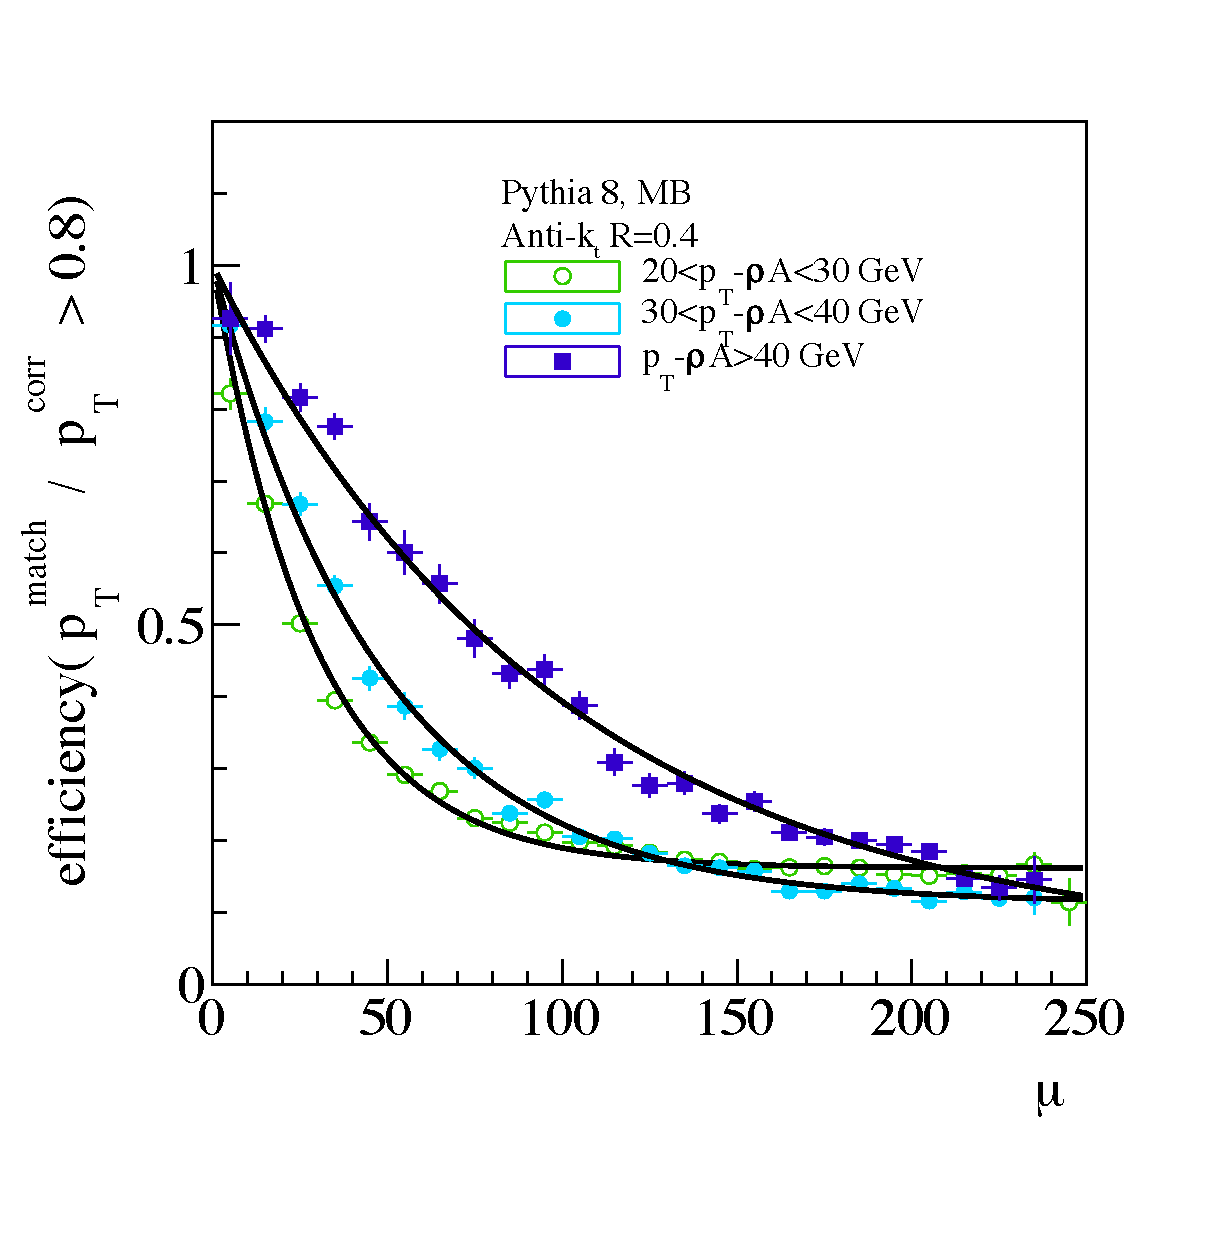
\includegraphics[width=0.46\textwidth]{20130710_frac_rpt_gt_0p8_vs_NPV_restricted_new.pdf}
    \caption[]{The fraction of \pujet s with $\Rpt > 0.8$ (QCD-like) as a function of the number of minimum-bias interactions  
    per event for different values of \ptcorr. A fit of the exponential form $f=c_0+c_1\exp(c_2\cdot N_{\rm PV})$ is superposed
    where one degree of freedom is fixed via the constraint $f(0)=1$, i.e. $c_1=(1-c_0)$.}
    \label{fig:FractionOfQCDlikePUjets}
  \end{center}
\end{figure}
%------------------------------



The contribution of particles from any vertex to a given \pujet{} can be measured using the jet vertex fraction (\JVF). It is defined as 
\begin{equation}
    \JVF(V_i) = \dfrac{\sum_{k = 1}^{\Npart(V_{i})} p_{\mathrm{T},k}}{\sum_{i=1}^{\Ncoll}\sum_{k=0}^{\Npart(V_{i})} p_{\mathrm{T},k}} = \dfrac{1}{\pT} \sum_{k = 1}^{\Npart(V_{i})} p_{\mathrm{T},k} ,
\label{eq:JVF}
\end{equation} 
where $\Npart(V_{i})$ is the number of particles from a given vertex $V_{i}$, and \Ncoll{} is the number of collision vertices contributing particles to the jet. \JVF{} is calculated for each of these vertices. 
Note that \pT\ corresponds to the uncorrected jet transverse momentum and consequently, the 
value of each component of $\JVF(V_i)$ depends on $\mu$. 
%%Fig.~\ref{fig:JVFexample} shows examples of the composition of two different jets in terms of \JVF.  In the context of this study \JVF{} is mainly used to illustrate the stochastic or QCD-like nature of \pujet s. The determination of the \pujet{} source is generally based on \Rpt, as discussed in the following section.  
%\begin{figure}[htbp!]
%  \begin{center}
%    \subfloat{\includegraphics[width=0.46\textwidth]{figures/JVFexample_1}\label{fig:JVFexample1}} \quad
 %   \subfloat{\includegraphics[width=0.46\textwidth]{figures/JVFexample_2}\label{fig:JVFexample2}}
  %  \caption[]{Example \JVF{} histograms for two \pujet s. In \subref{fig:JVFexample1}, the constituents emerging
  %              from three vertices contribute in a comparable amount to the total jet \pT. About $90\%$ of the jet \pT{} arises from only one \MB{} interaction in the jet shown in \subref{fig:JVFexample2}.}
 %   \label{fig:JVFexample}
%  \end{center}
%\end{figure}


\subsection{Evaluation of the \pu{} jet nature}


It follows from the definition of \Rpt{} that \pujet s with values of \Rpt{} close to unity are matched to a truth jet with $\pT \approx \ptcorr$ of the \pujet{} itself. Consequently, there is a single \MB{} interaction which predominantly contributes to the jet. On the other hand, jets with a small value of \Rpt{} are mostly stochastic, as no single minimum-bias collision contributes in a dominant way to the \pujet. We characterize jets as stochastic if \Rpt{} is smaller than 0.8. This threshold value is arbitrary and the fraction of QCD-like and stochastic jets depends on the exact choice. The conclusion of our study holds for a broad range of cut values.
%------------------------------
%\begin{figure}[htbp!]\centering
%\subfigure[$20 < \pT - \rho A < 25$~\GeV]{\includegraphics[width=0.46\textwidth]%
%{figures/20130710_pttruePverptcorr_ptcorr_20to25_new.pdf}\label{fig:pttrueOverPtcorr:0}} \qquad
%\subfigure[$\pT - \rho A > 30$~\GeV]{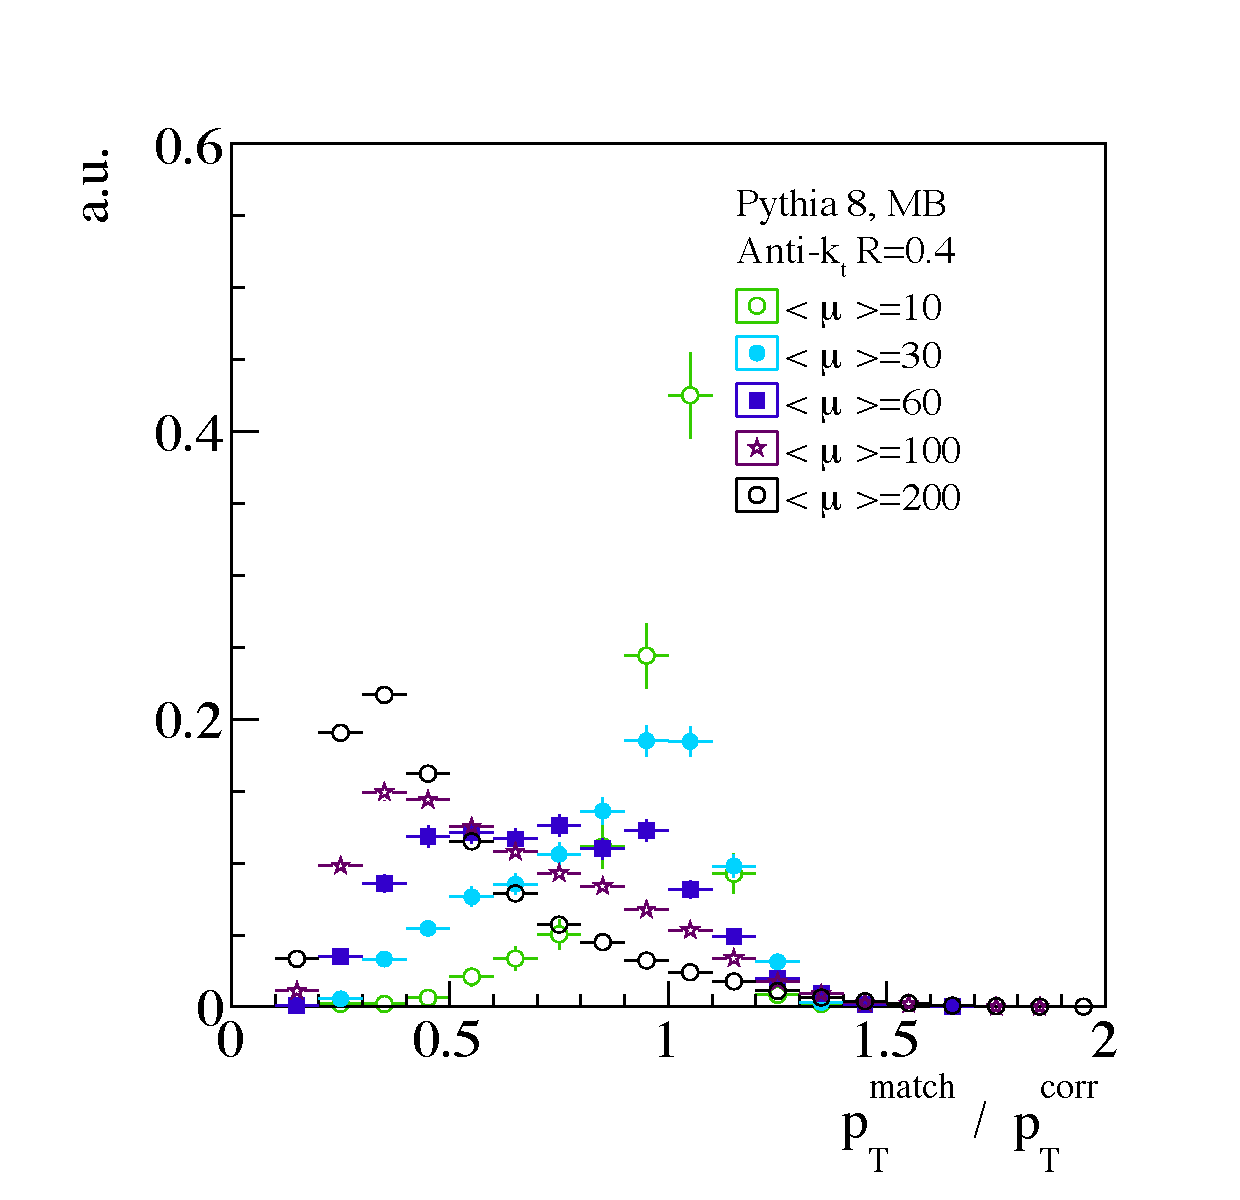
\includegraphics[width=0.46\textwidth]{figures/20130710_pttruePverptcorr_ptcorr_gt30_new.pdf}\label{fig:pttrueOverPtcorr:1}}
%\caption[]{ The distribution of \Rpt, as given in Equation~\ref{eq:match}, for \pujet s with different ranges of $\pt - \rho A$,
%                   for different \axing{}. The cutoff on the low side of \Rpt{}% is due
 %               to the $\ptmatch > 5\GeV$ requirement.}
 %   \label{fig:pttrueOverPtcorr}
%\end{figure}
%------------------------------


%%This interpretation of different \Rpt{} values in stochastic and QCD-like jets is illustrated in Figures~\ref{fig:jvf_rpt}\subref{fig:JVF_Rpt_lt_0.3:0} to \subref{fig:JVF_Rpt_0.8:1}.
%\begin{figure}[htbp!]\centering
%\subfloat[$\Rpt = 0.29$, $\ptcorr = 20.6$~\GeV, $<\mu> = 20$]
%	{\includegraphics[angle=90,width=0.46\textwidth]{figures/20130628_JVF_Rpt_lt0p3_mu20.pdf}\label{fig:JVF_Rpt_lt_0.3:0}} \qquad
%\subfloat[$\Rpt = 0.20$, $\ptcorr = 25.0$~\GeV, $<\mu> = 120$]{\includegraphics[angle=90,width=0.46\textwidth]{figures/20130628_JVF_Rpt_lt0p3_mu120.pdf}\label{fig:JVF_Rpt_lt_3.0:1}}
%\quad
%\subfloat[$\Rpt = 0.85$, $\ptcorr = 21.0~$\GeV, $<\mu> = 20$]
%	{\includegraphics[angle=90,width=0.46\textwidth]{figures/20130628_JVF_Rpt_gt0p8_mu20.pdf}\label{fig:JVF_Rpt_gt_0.8:0}} \qquad
%\subfloat[$\Rpt = 0.88$, $\ptcorr = 23.1$~\GeV, $<\mu> = 120$]{\includegraphics[angle=90,width=0.46\textwidth]{figures/20130628_JVF_Rpt_gt0p8_mu120.pdf}\label{fig:JVF_Rpt_0.8:1}}
%\caption[]{\JVF{} distributions for \pujet s with similar corrected kinematics but at different levels of \pu{} and for lower (\subref{fig:JVF_Rpt_lt_0.3:0} and \subref{fig:JVF_Rpt_lt_3.0:1}) and higher (\subref{fig:JVF_Rpt_gt_0.8:0} and \subref{fig:JVF_Rpt_0.8:1}) \Rpt{} values.\label{fig:jvf_rpt}}
%\end{figure}
%------------------------------

The fractions of QCD-like and stochastic \pujet s change as a function of pileup jet \pt{} and $\mu$. This can be seen in Fig.~\ref{fig:FractionOfQCDlikePUjets}, where \qcdjet-like
samples are defined by $\Rpt > 0.8$ for each \pu{} level. The fraction of these jets at a given \ptcorr{} decreases exponentially with $\mu$.  The exponential decrease is slower for larger the \ptcorr. 
At a \pu{} activity of $\mu=100$, the fraction of \pujet{}s that are QCD-like is about 40\% (20\%) for $\ptcorr > 40\GeV$ ($20 < \ptcorr <30\GeV$). At  $\mu=150$, these numbers
decrease to about 25\% and 15\%, respectively. 
 


\subsection{\PU{} jet multiplicity}
The mean number of pileup jets per event, as a function of jet \ptcorr~and 
$N_{\rm PV}$, is indicative of the efficiency of the jet area based method to suppress jets generated by \pu. It is shown in Fig.~\ref{fig:pujetmult} for the inclusive \pujet s and separately for the subsample of QCD-like \pujet s satisfying $\Rpt  > 0.8$. It is observed that the average inclusive number $\langle N\rangle$ of low ($\ptcorr \simeq 20\GeV$) \pujet s per event increases rather linearly with $\mu$, i.e. $\partial \langle N \rangle/\partial \mu \approx \mathrm{const}$. For higher \pujet{} \pT, $\partial \langle N \rangle/\partial \mu$ is significantly smaller, and displays an increase with increasing $\mu$.

The sub-sample of QCD-like jets in the inclusive \pujet{} sample shows a different behavior, as indicated in the righmost panel of Fig.~\ref{fig:pujetmult}. In this case $\partial \langle N \rangle/\partial \mu$ decreases with increasing $\mu$ in all considered bins of \ptcorr. This contradicts the immediate expectation of an increase following the inclusive sample, but can be understood from the fact that with increasing $\mu$ the likelihood of QCD-like jets to overlap with (stochastic) jets increases as well. The resulting (merged) \pujet s no longer display features consistent with \qcdjet s (e.g., loss of single energy core), and thus fail the $\Rpt > 0.8$ selection.

\begin{figure*}[htbp!]\centering
\subfigure[]{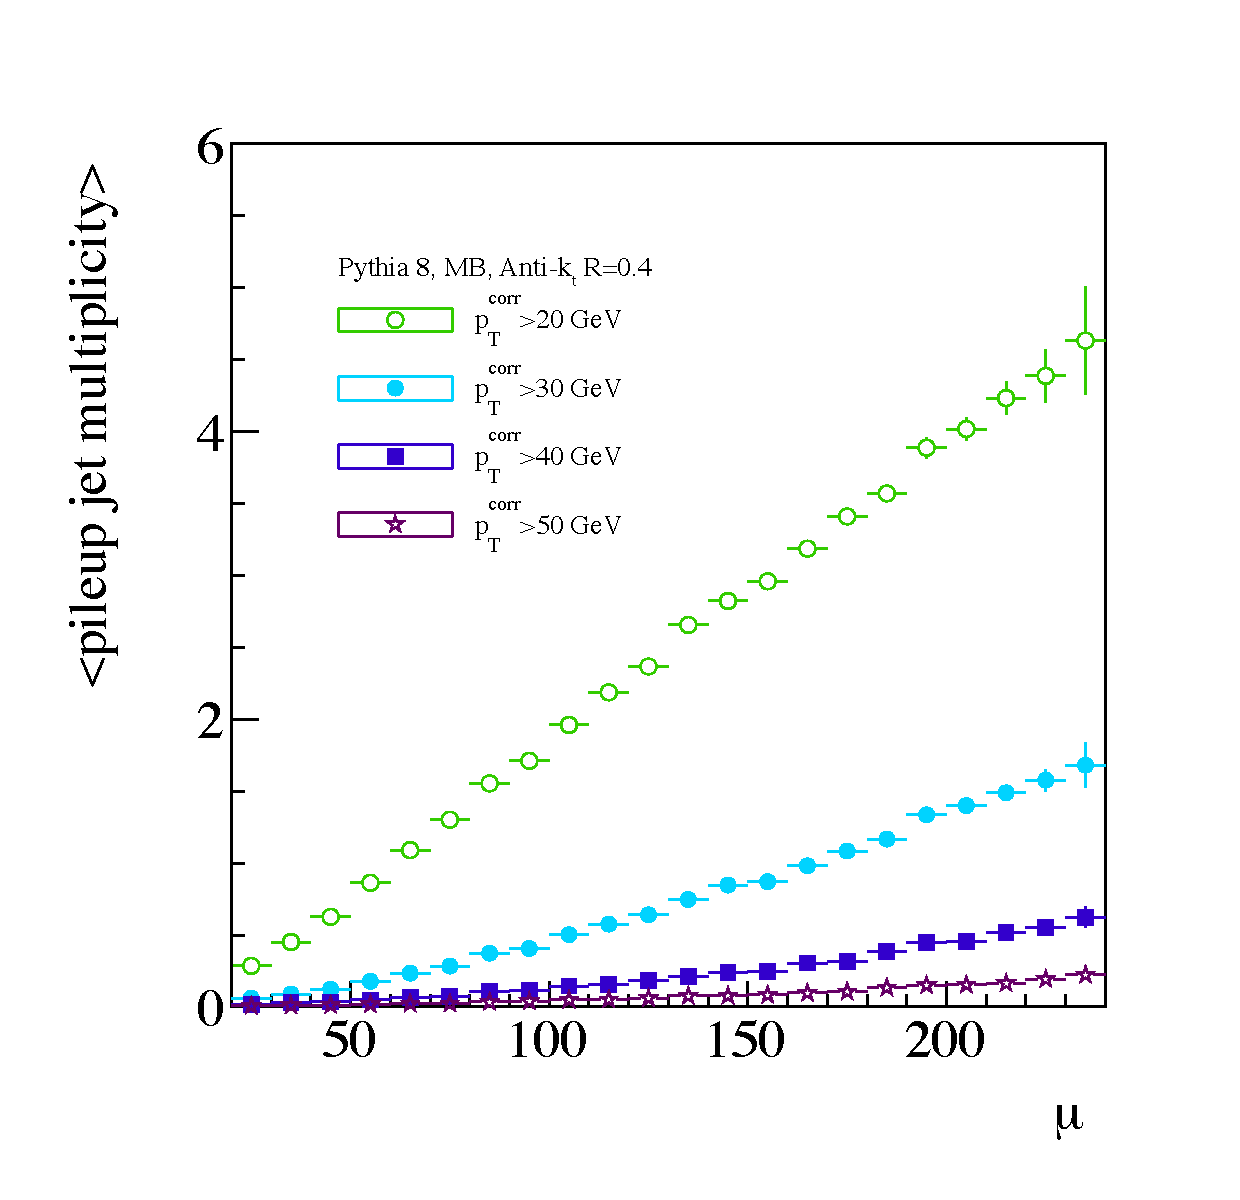
\includegraphics[width=0.46\textwidth]{20130710_PUjetmult_inc_new.pdf}\label{fig:pujetmult:0}}
\subfigure[]{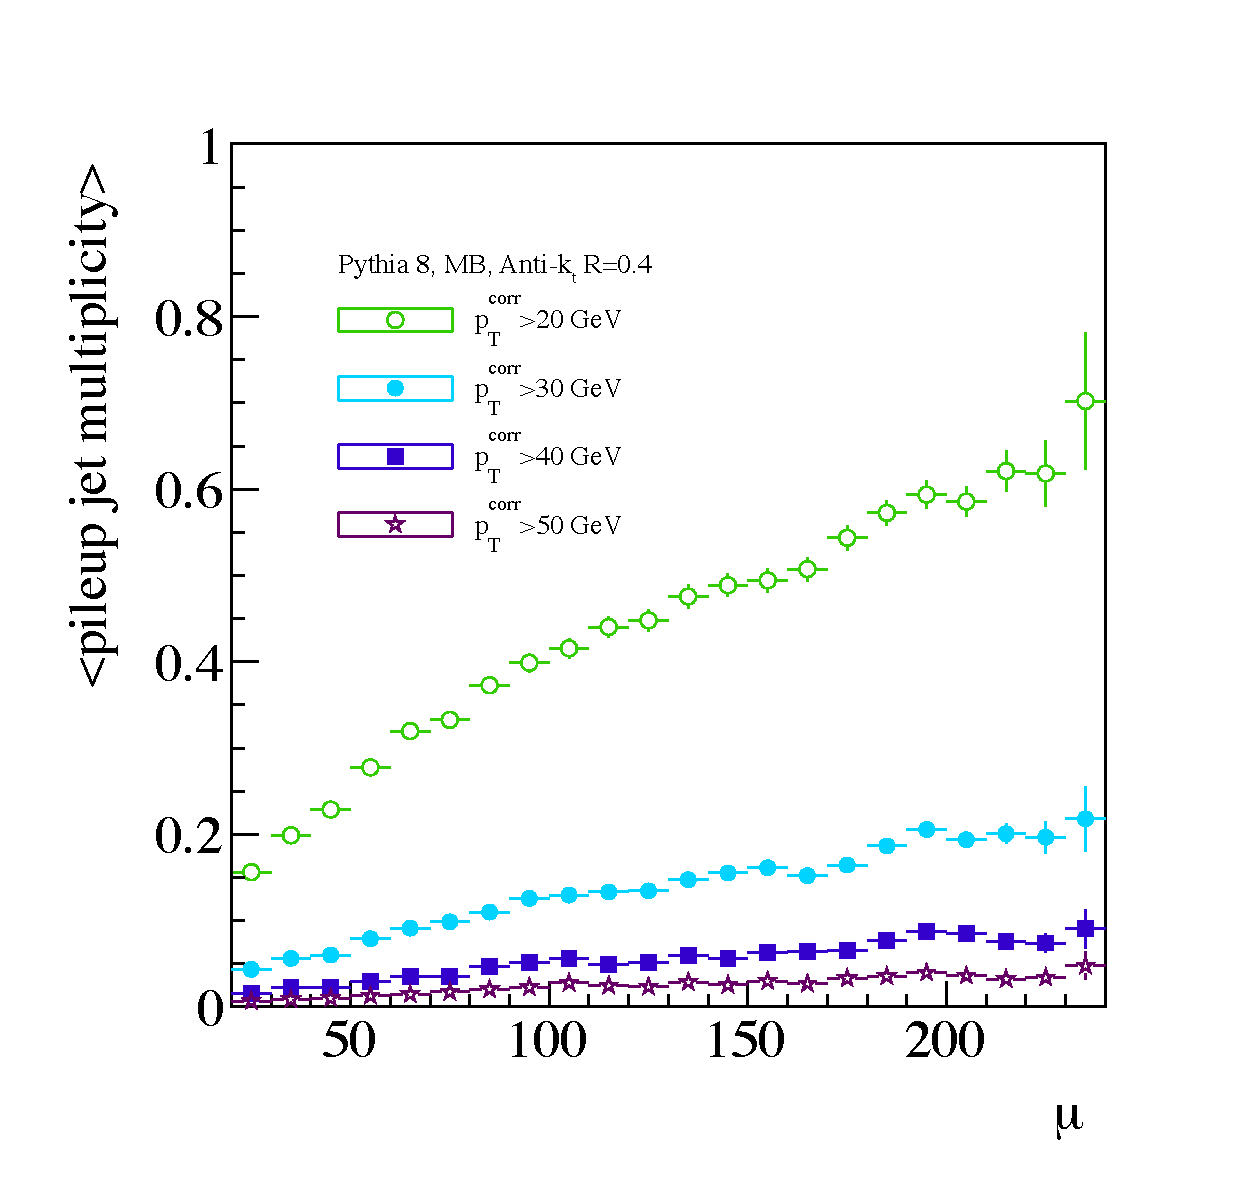
\includegraphics[width=0.46\textwidth]{20130710_PUmult_Rptgt0p8_new.pdf}\label{fig:pujetmult:1}}
    \caption[]{The mean number of pileup jets per event inclusively \subref{fig:pujetmult:0} and for QCD-like pileup jets with $\Rpt > 0.8$
    \subref{fig:pujetmult:1}, as a function of $\mu$ and \ptcorr. }
    \label{fig:pujetmult}
\end{figure*}
%-----------------------

The \pujet{} multiplicity shown in Fig.~\ref{fig:pujetmult} is evaluated as a function of the \pu{} corrected transverse momentum of the jet (\ptcorr). This means that after the correction approximately two \pujet{}s with $\ptcorr > \pTmin = 20$~\GeV{} can be expected for $\axing \simeq 100$. This number decreases rapidly with increasing \pTmin. The mean number of \qcdjet s is small, at about 0.4 at $\axing = 100$, for $\pTmin = 20$~\GeV.

%%\subsection{Concluding remarks about \pu{} jets}


%\bibliographystyle{boostnote}
%\bibliography{boostbib}















%\subsection{Study of grooming performance in the presence of large pile-up at the LHC} \label{sec:intro}

%The kinematic domains newly reachable with \pp{} collisions taken both
%at \sqrts{7} (2011) and \sqrts{8} (2012) \cms{} energies at the \LHC{}
%allow investigations of final states with highly boosted heavy
%particle decays. These decays are characterized by the feature that
%all the decay products can be reconstructed within one jet with a
%radial distance parameter $R \approx 2M/\pT$, where $M$ is the mass of
%the decaying particle, and \pT{} is its transverse momentum. So far
%boosted heavy objects reconstructed in the available data from
%\ATLAS{} \cite{Aad:2008zzm} and \CMS{} \cite{Chatrchyan:2008aa} are
%hadronically decaying \Wboson{} bosons, and fully hadronic top-quark
%decays (see e.g. Refs.~\cite{Chatrchyan:2012ku,Aad:2012dpa}).
%
% The ultimate application of the jet grooming techniques used in this
% reconstruction, all of which are based on the enhancement of the two
% or three prong structure of the decay over the parton shower and
% fragmentation driven jet structures for light quark and gluon
% originated jets, is in searches for new physics with new heavy
% particles that decay into boosted hadronic final states.
%
%The ultimate application of the jet substructure techniques used in
%these reconstructions, based on the enhancement of the two or three
%prong structure of the decay over the parton shower and fragmentation
%driven jet structures for light quark and gluon originated jets, is in
%searches for new physics with new heavy particles decay into boosted
%hadronic final states. In this picture, grooming techniques aim at
%reducing the sensitivity to the soft radiation while keeping the hard
%prongs in the fat jet, resulting in a better resolution and improved
%signal-to-background ratios.





%%In Section \ref{sec:events} of this article the Monte Carlo event
%%generation is described, together with the pile-up modeling. In
%%addition, the basic analysis tools are presented. In the following
%%Section \ref{sec:grooming} the applied jet grooming techniques and
%%their specific configurations are discussed. The results for the top
%%mass are presented in Section \ref{sec:results}, followed by brief
%%conclusions in Section \ref{sec:concl}.
 
%\subsection{Event generation and analysis}\label{sec:events}

\subsection{Jet grooming configurations} \label{sec:grooming}

Three jet grooming techniques are used by the LHC experiments:
\begin{description}
\item{\textbf{Jet trimming}} Trimming is described in detail in Ref.~\cite{Krohn:2009th}. In this approach the constituents of the large \antikt{} jet formed with $R = 1.0$ are re-clustered into smaller jets with $R_{\mathrm{trim}} = 0.2$, using the \antikt{} algorithm again. The resulting sub-jets are only accepted if their transverse momentum is larger than a fraction $f$ (here $f = 0.03$) of a hard scale, which was chosen to be the \pT{} of the large jet. The surviving sub-jets are recombined into a groomed jet.
\item{\textbf{Jet filtering}} Filtering was introduced in the context
  of a study to enhance the signal from the Higgs boson decaying into
  two bottom-quarks, see Ref.~\cite{Butterworth:2008iy}. In its
  simplified configuration without mass-drop criterion~\cite{Cacciari:2008gd} 
  applied in this study it works
  similar to trimming, except that in this case the sub-jets are found
  with the Cambridge-Aachen algorithm
  \cite{Wobisch:1998wt,Wobisch:2000dk} with $R_{\mathrm{filt}} = 0.3$,
  and only the three hardest sub-jets are retained. The groomed jet is
  then constructed from these three sub-jets.   
\item{\textbf{Jet pruning}} Pruning was introduced in
  Ref.~\cite{Ellis:2009su}. Contrary to filtering and trimming, it
  is applied during the formation of the jet, rather than based on
  the recombination of sub-jets. It dynamically suppresses small
  and larger distance contributions to jet using two parameters,
  $Z_{\mathrm{cut}}$ for the momentum based suppression, and
  $D_{cut} = D_{\mathrm{cut,fact}} \times 2 m/\pT$ (here $m$ and
  \pT{} are the transverse momentum and mass of the original jet)
  for the distance based. Pruning vetoes
  recombinations between two objects $i$ and $j$ for which the
  geometrical distance between $i$ and $j$ is more than $D_{\rm cut}$
  and the $p_T$ of one of the objects is less than $Z_{\rm cut}
  \times p_T^{i+j}$, where $p_T^{i+j}$ is the combined transverse
  momentum of $i$ and $j$. In this case, only the hardest of the two
  objects is kept. Typical values for the parameters are: 
  $Z_{\mathrm{cut}} = 0.1$ and
  $D_{\mathrm{cut,fact}} = 0.5$.
\end{description} 

In this study, trimming and filtering are applied to the original \antikt{} jets with size $R = 1.0$. 
%
%The subtraction is performed using the four-momentum area defined in \FJ.
%on the \pT{} scale and then applied to the mass scale,
%\begin{equation}
%p_{\mathrm{T,corr}} = \max(0, \pT - A_{\mathrm{jet}} \times \rho) \Rightarrow m_{\mathrm{corr}} = \dfrac{p_{\mathrm{T,corr}}}{\pT} m\, . 
%\label{eq:pusubs}
%\end{equation} 
%Here $A_{\mathrm{jet}}$ is the catchment area of the jet, defined as
%suggested in Ref.~\cite{Cacciari:2008gn}. 
%
We study the interplay between jet grooming and area-based pile-up 
correction. The subtraction is applied directly on the 4-momentum 
of the jet using:
\begin{equation}\label{eq:pusub}
  p^\mu_\text{jet,sub} = p^\mu_\text{jet}  
  - [\rho A^x_\text{jet}, \,\rho A^y_\text{jet}, \,
  (\rho+\rho_m) A^z_\text{jet}, \,(\rho+\rho_m) A^E_\text{jet}]\,,
\end{equation}
with
\begin{equation}
  \rho = \mathop{\text{median}}_\text{patches}
  \left\{\frac{p_{t,\text{patch}}}{A_\text{patch}}\right\}
  \,,\quad
  \rho_m = \mathop{\text{median}}_\text{patches}
  \left\{\frac{m_{\delta,\text{patch}}}{A_\text{patch}}\right\},
\end{equation}
$m_{\delta,\text{patch}} = \sum_{i\in\text{patch}}
\big(\sqrt{\smash[b]{m^2_{i} + p_{t,i}^2}} - p_{ti}\big)$, and $A^\mu$
is the active area of the jet as defined in
Ref.~\cite{Cacciari:2008gn} and computed by FastJet. The $\rho$ term,
mentioned above is the standard correction typically correcting the
transverse momentum of the jet. The $\rho_m$ term corrects for
contamination to the total jet mass due to the PU particle. 
When applying this subtraction procedure, we
discard jets with negative transverse momentum or (squared) mass of the jet.
%

\begin{figure*} [p!]
\begin{center}
\subfigure[raw, ungroomed jets]{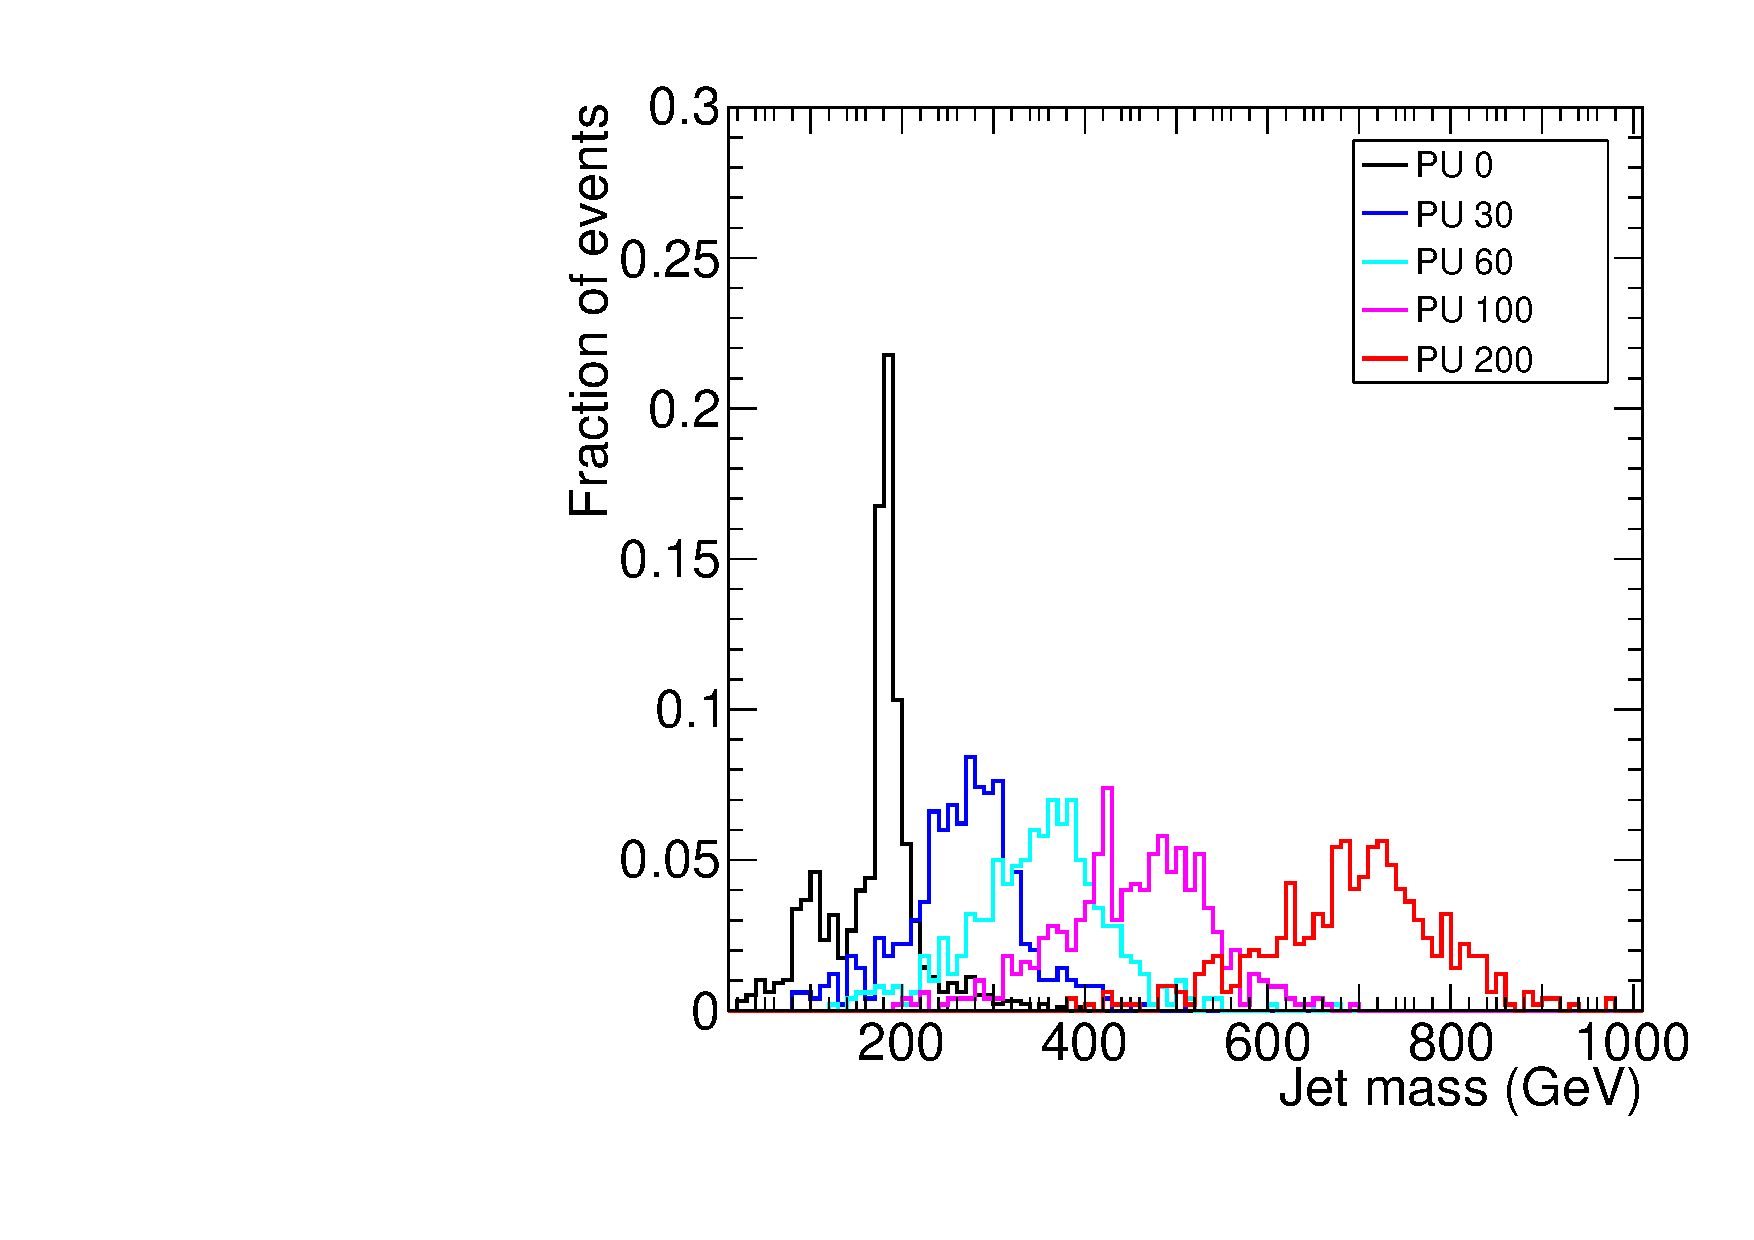
\includegraphics[width=0.4\textwidth]{comparePUs_ak10_noPUsub}}
\subfigure[raw jets with pile-up subtraction]{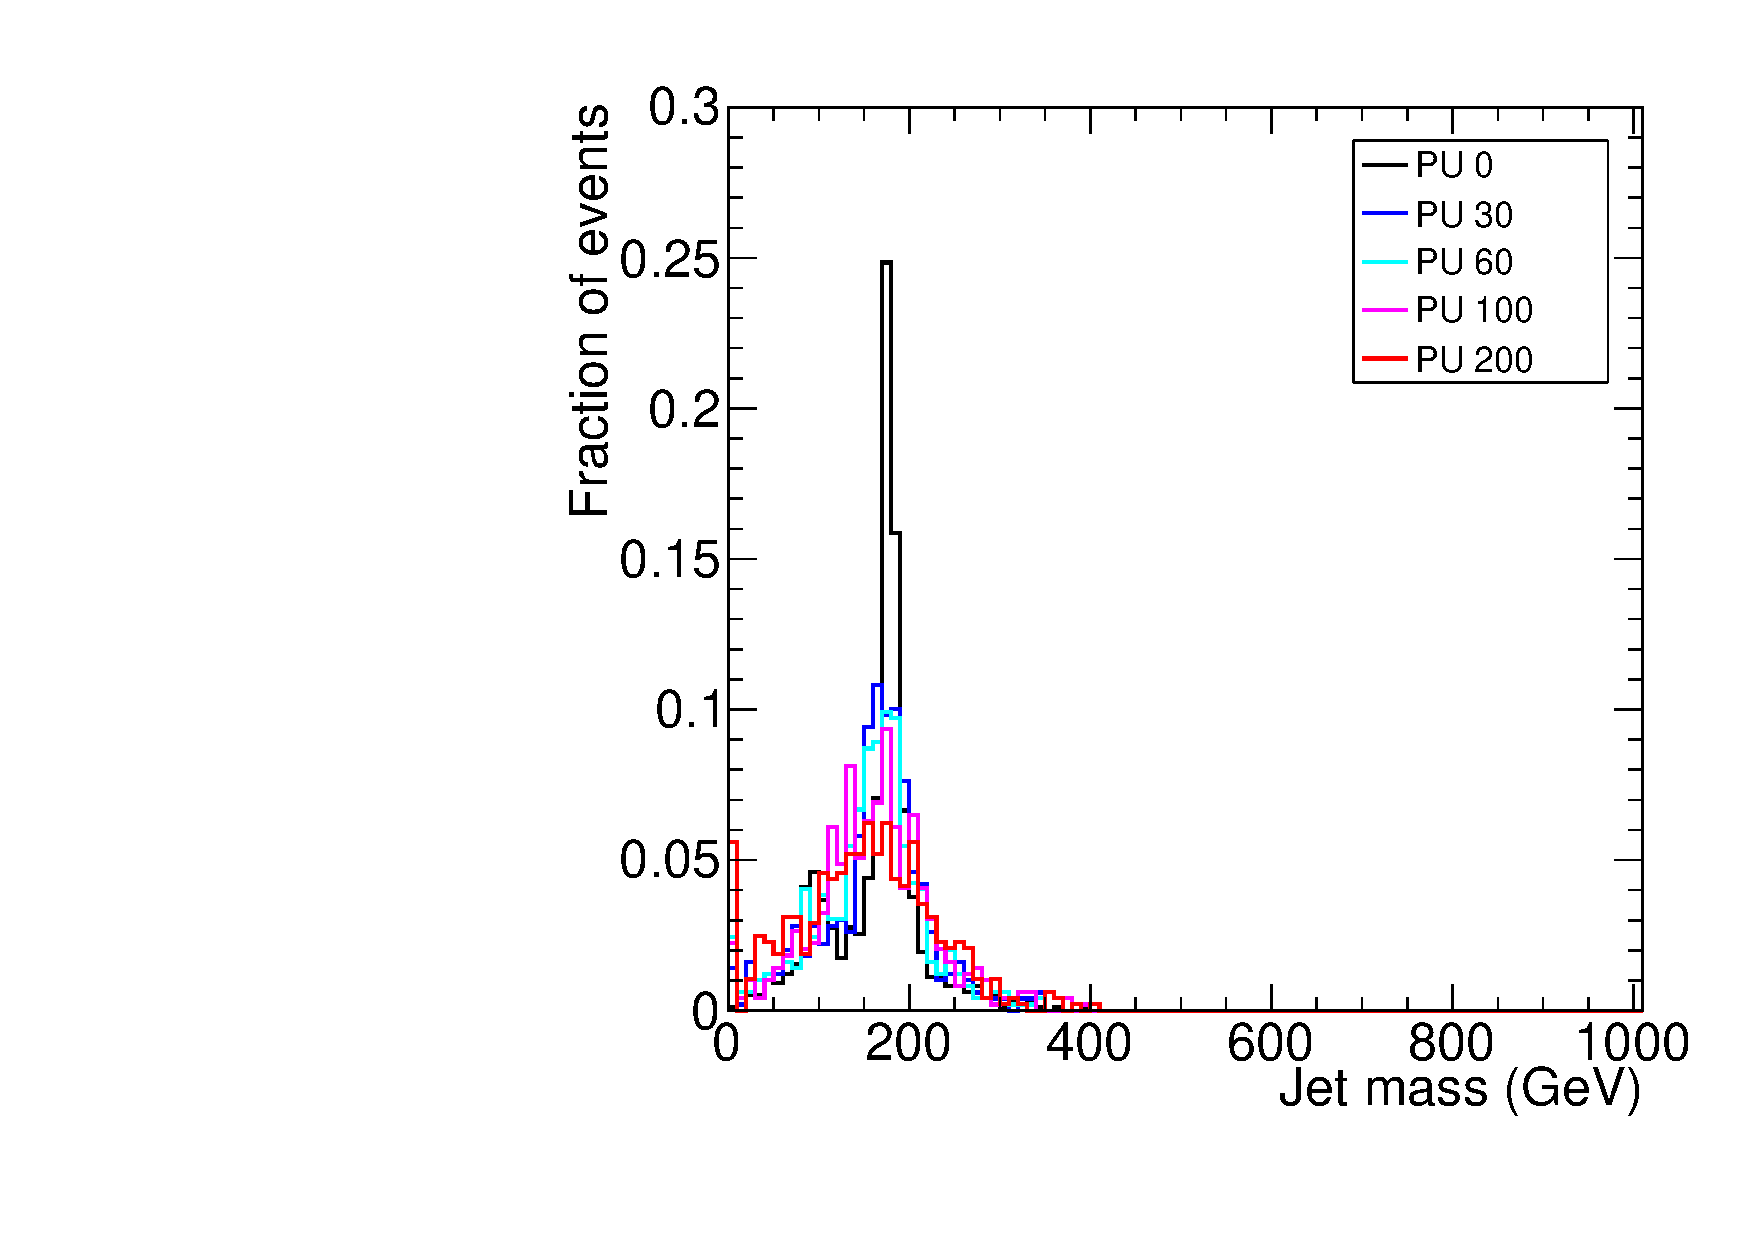
\includegraphics[width=0.4\textwidth]{comparePUs_ak10_PUsub}}
\subfigure[trimmed jets]{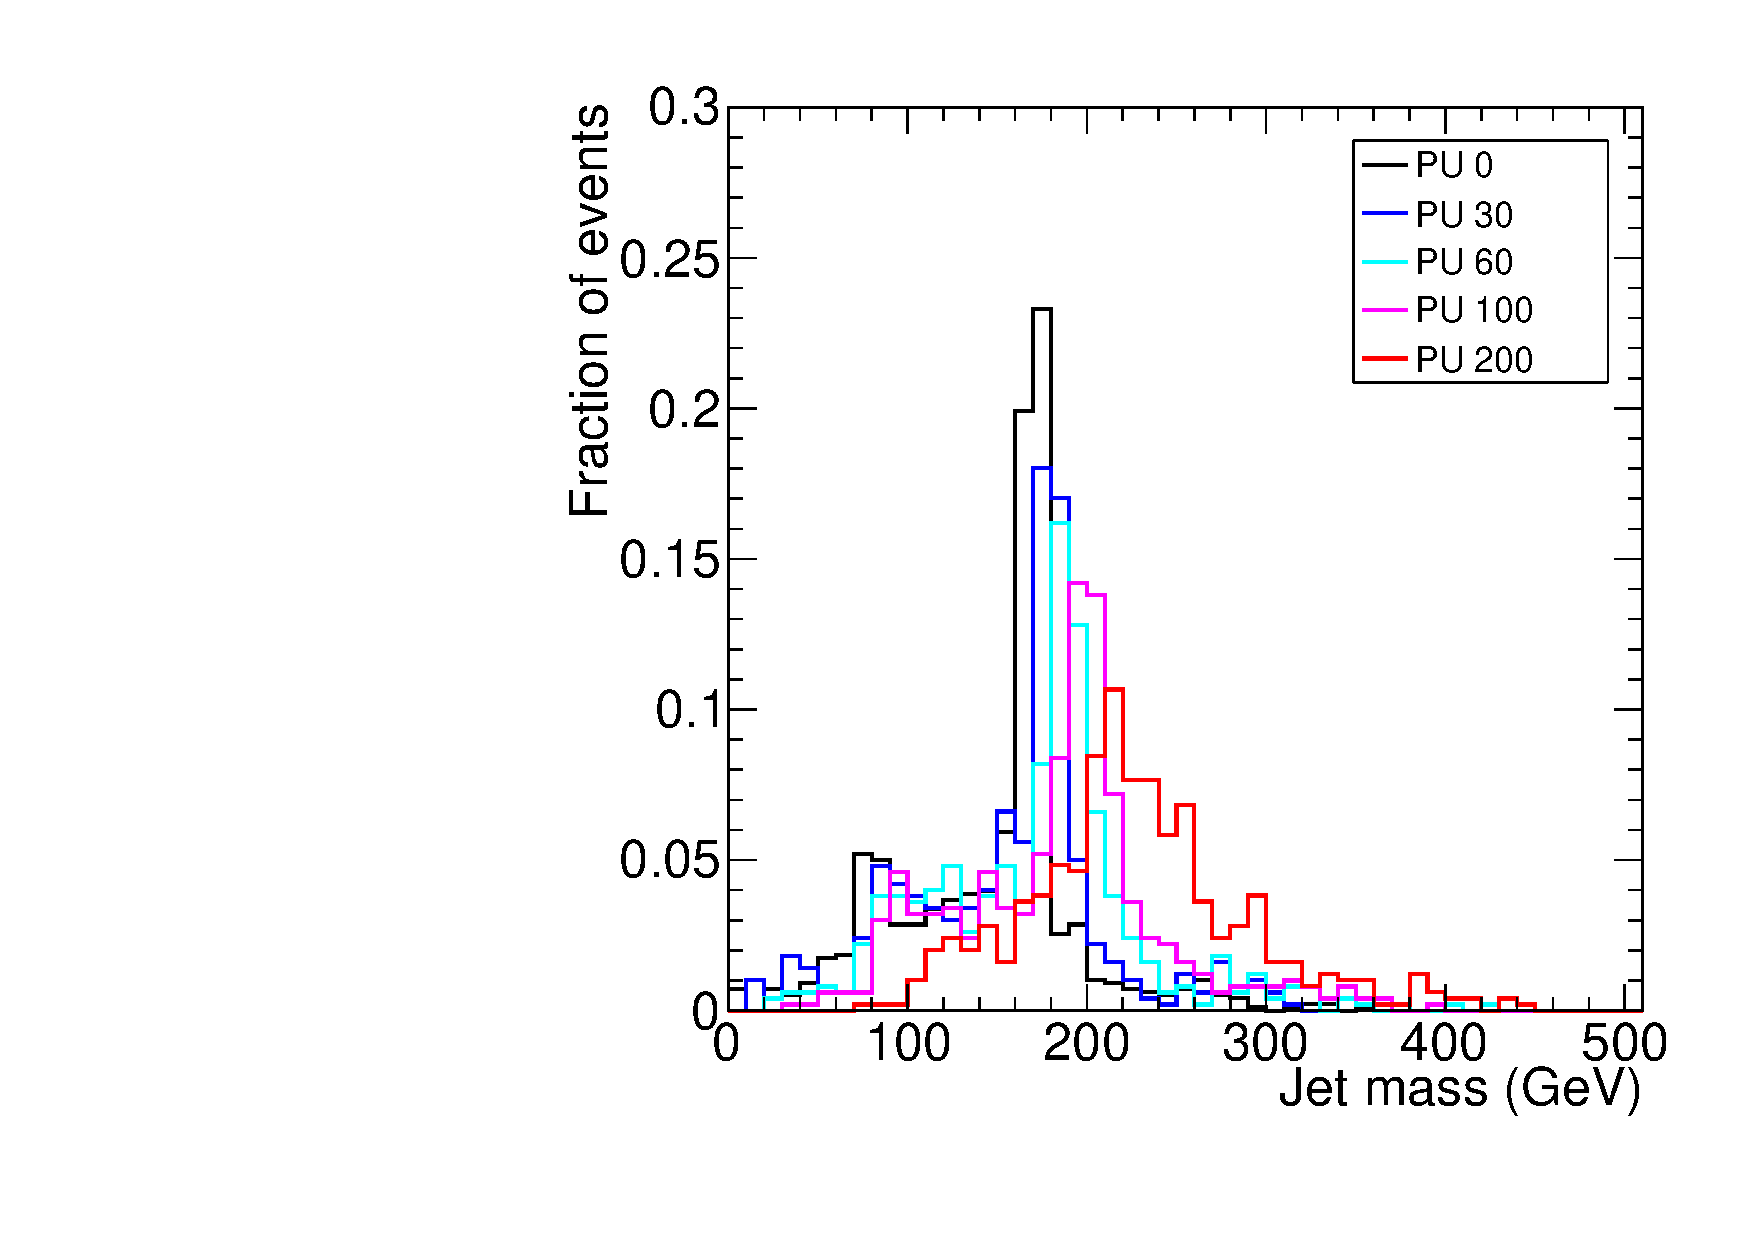
\includegraphics[width=0.4\textwidth]{comparePUs_ak10_tr_noPUsub}} 
\subfigure[trimmed jet with pile-up subtraction]{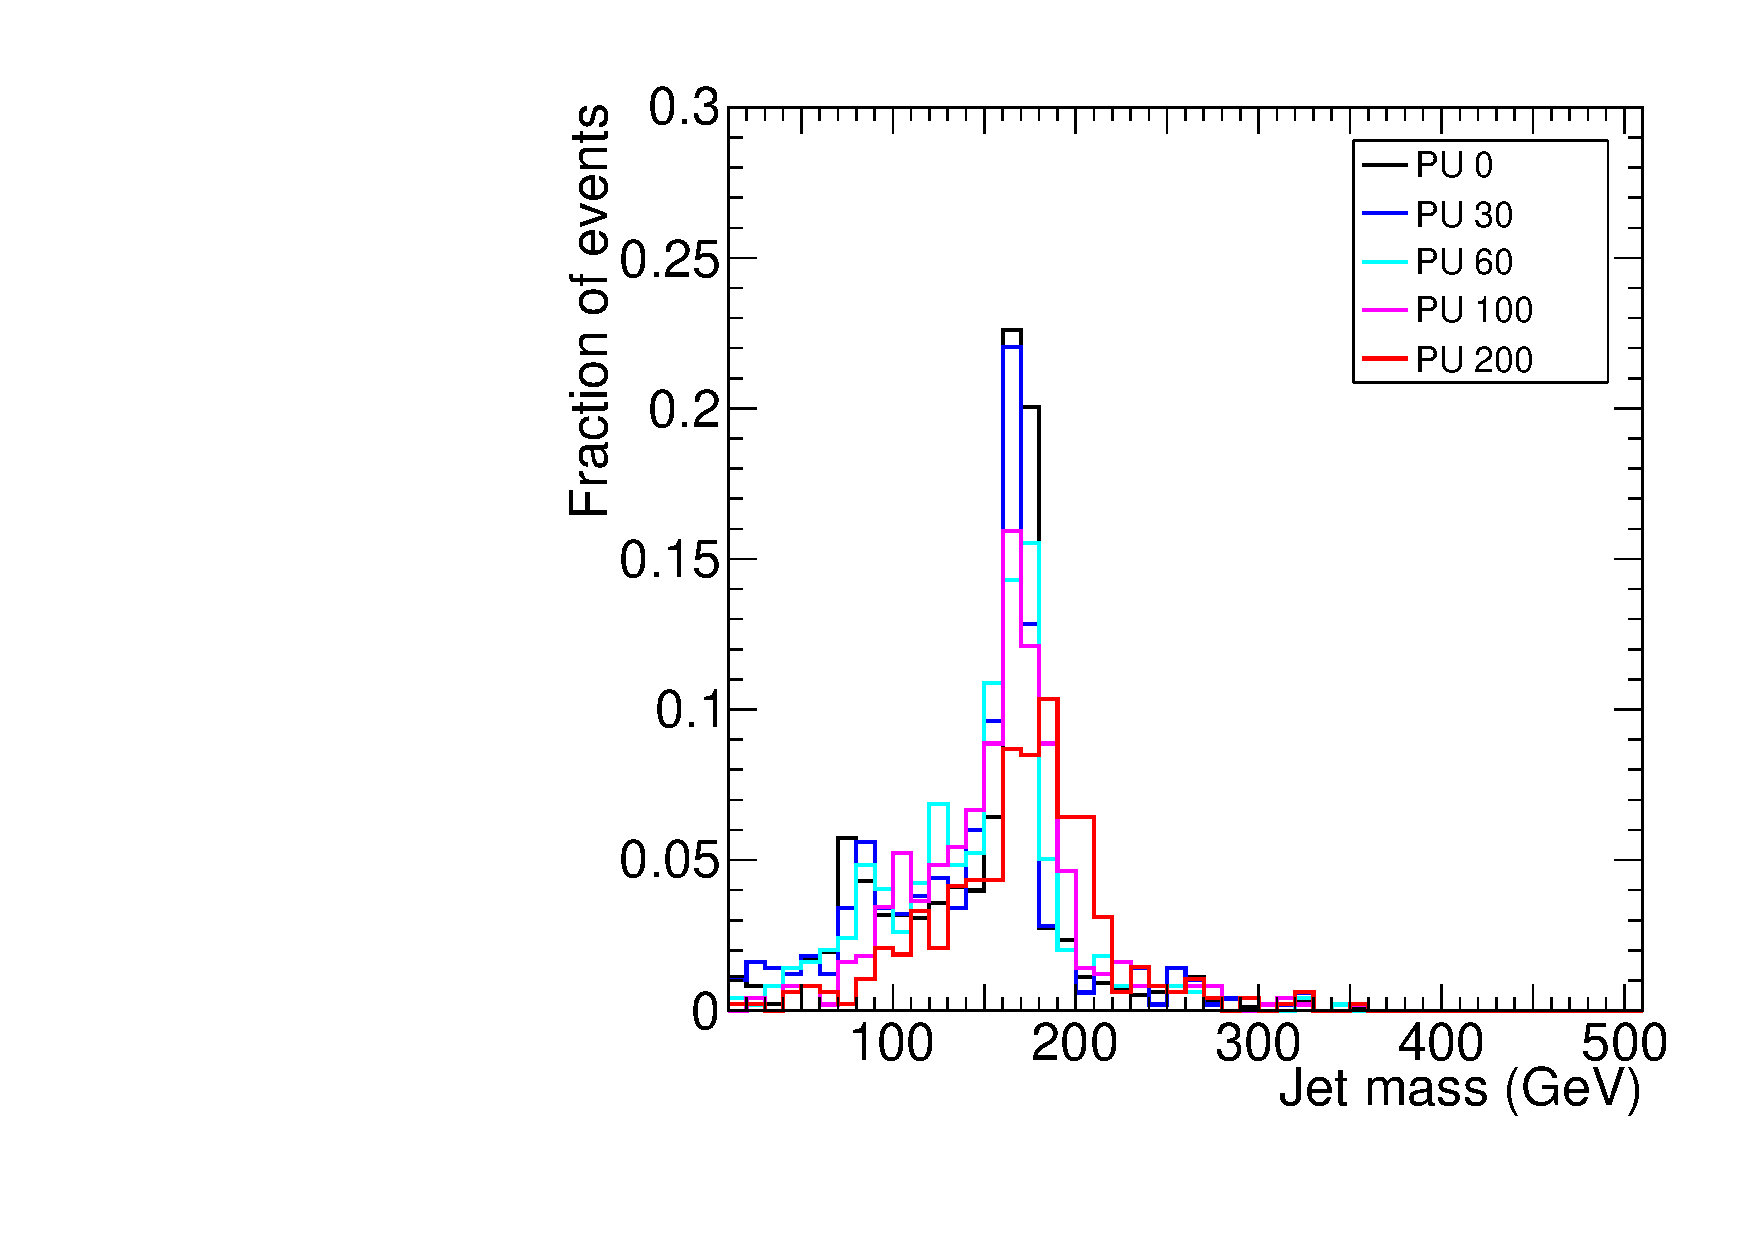
\includegraphics[width=0.4\textwidth]{comparePUs_ak10_tr_PUsub}}
\subfigure[filtered jets]{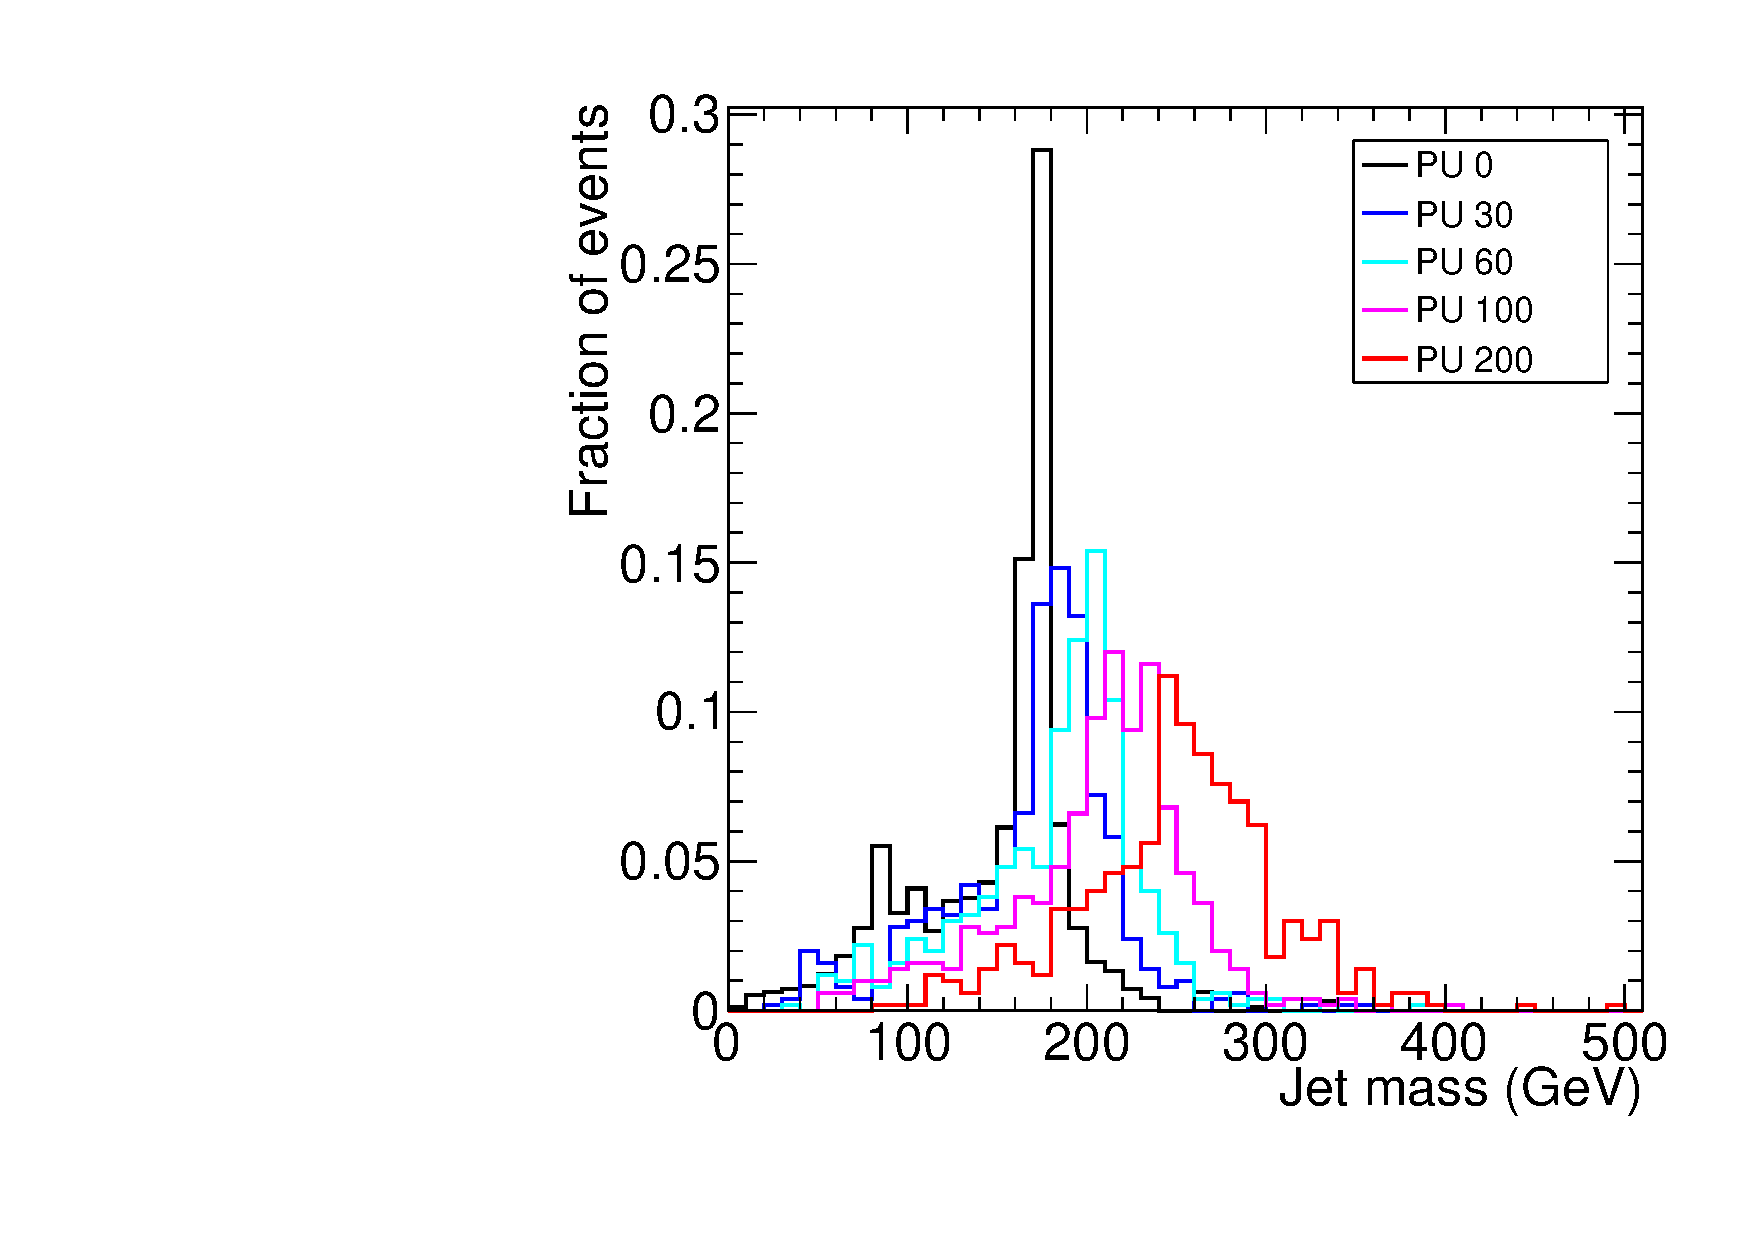
\includegraphics[width=0.4\textwidth]{comparePUs_ak10_ft_noPUsub}}
\subfigure[filtered jet with pile-up subtraction]{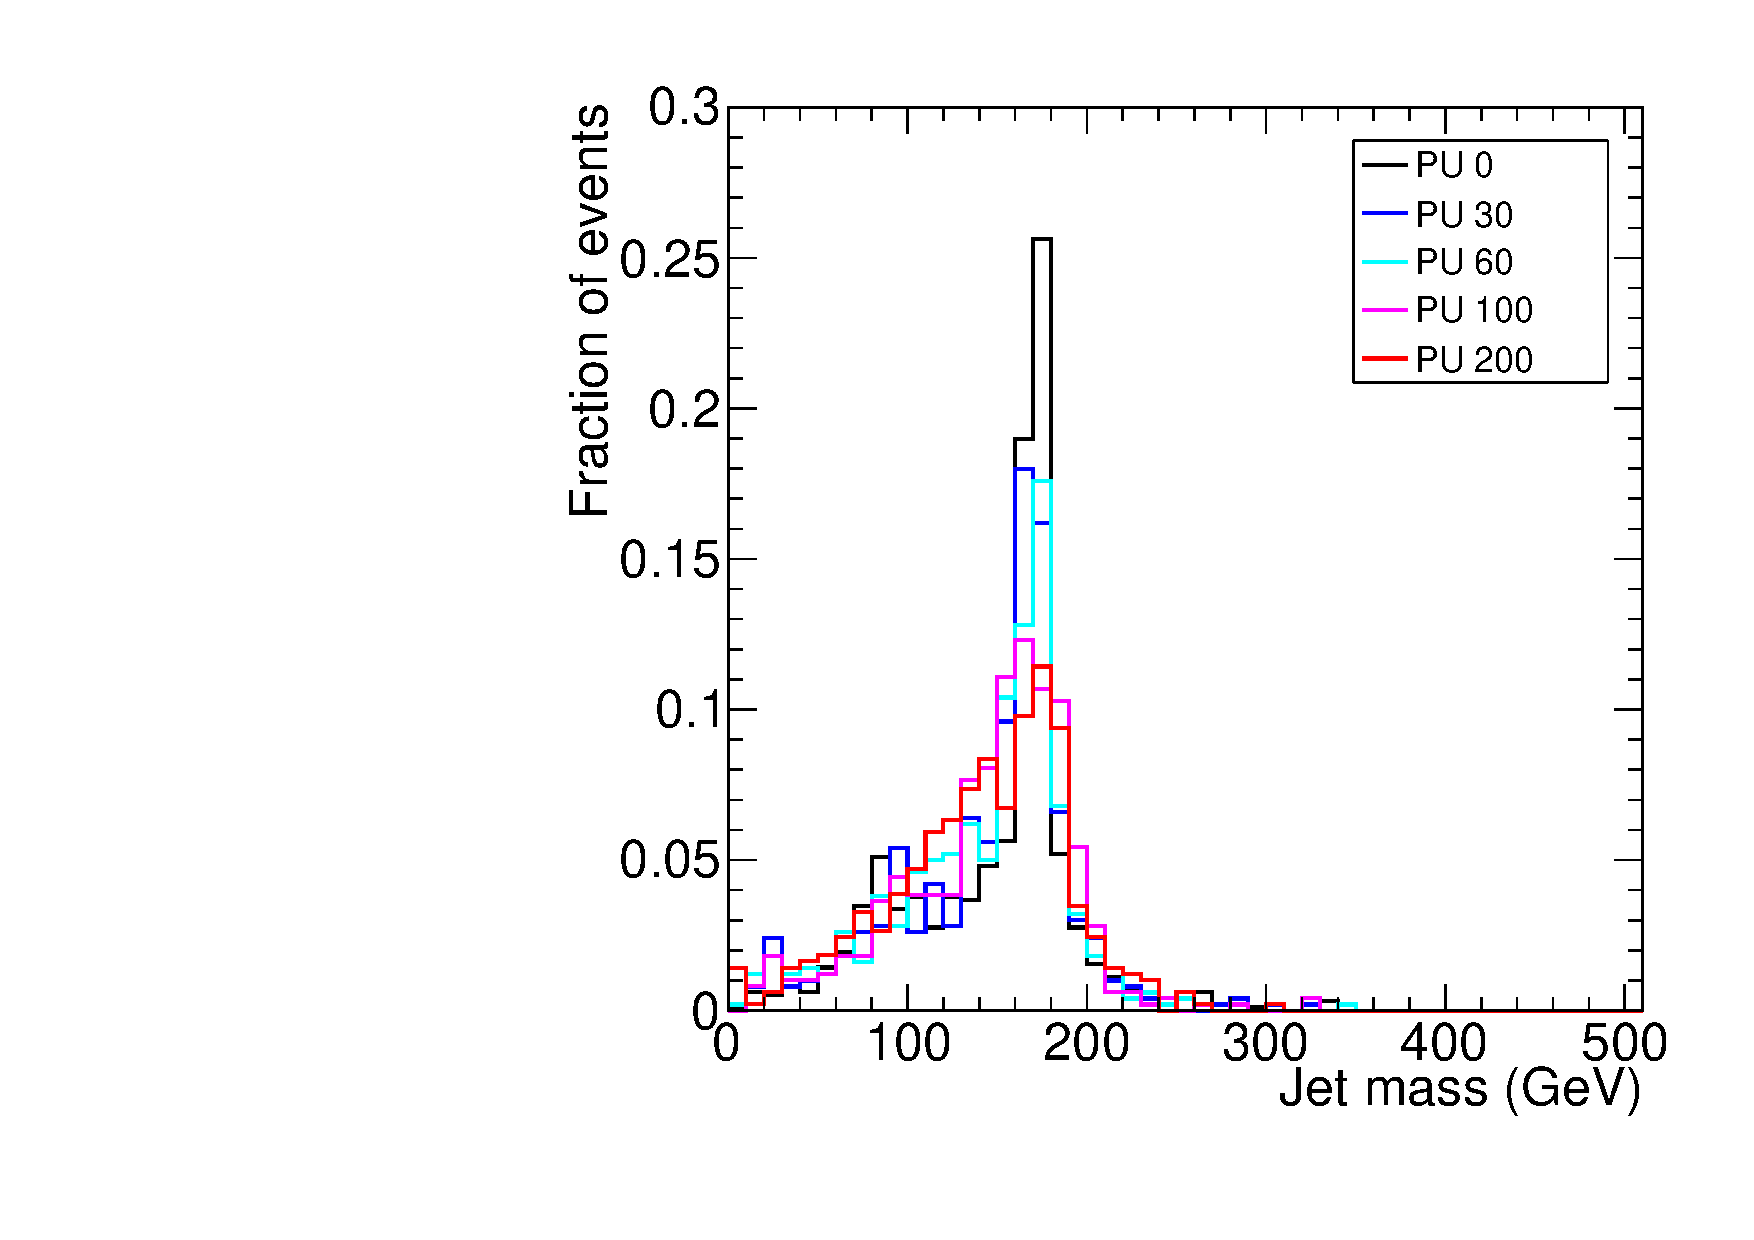
\includegraphics[width=0.4\textwidth]{comparePUs_ak10_ft_PUsub}} 
\end{center}
\caption[]{The impact of \pu{} on the jet mass distribution. Top row: the raw jet mass distribution for jets reconstructed with the \antikt{} algorithm and $R = 1.0$ in $\Zprime \to \ttbar$ final states with $m_{Z'} =$ 1.5~\tev{}, in the presence of pile-up with $\axing = 30$, 60, 100, and 200, before and after pile-up subtraction. The second and third row show the same result after trimming (middle row) and filtering (lower row).}
\label{fig:mass_spectra}
\end{figure*}

The estimation of $\rho$ and $\rho_m$ is performed with \FJ\ 
using\footnote{Ghosts
  are placed up to $y_{\rm max}=3$ and explicit ghosts are enabled.}
$k_t$ jets with $R=0.4$. Corrections for the rapidity dependence of
the pileup density $\rho$ are applied using a rapidity rescaling.

When we apply this background subtraction together with trimming or
filtering, the subtraction is performed directly on the subjets,
before deciding which subjets should be kept, so as to limit the
potential effects of pileup on which subjets are to be kept.

\subsection{Jet substructure performance}
\label{sec:results}

%\begin{figure*} [h!]
%\begin{center}
%
%\end{center}
%\caption{Jet mass spectra for jets reconstructed with the \antikt{} algorithm and $R = 1.0$ in $\Zprime \to \ttbar$ final states, in the presence of pile-up with $\axing = 30$, 60, 100, and 200. The distributions in the leftmost plot are for the uncorrected jet masses, the rightmost plot corresponds to the jet mass distributions after pile-up subtraction.}
%\label{fig:mass_spectra1}
%\end{figure*}  





The various methods and configurations discussed in the previous
section are applied to the jets reconstructed with the \antikt{}
algorithm with $R = 1.0$ in the $\Zprime \to \ttbar$ final state in
the presence of pile-up. For the studies presented in this report we require
jet \pT{} before grooming and pileup subtraction to be greater than 100
GeV and consider the two hardest \pT jets in the event. We further
require that the rapidity difference between the two jets $|y_1 -
y_2|$ is less than one.
%
The immediate expectation for the reconstructed jet mass $m$ is the
top mass, i.e. $m \approx 175$~\GeV, and no residual dependence on the
pile-up activity given by \axing, after the pile-up
subtraction. The two plots in the upper row of 
Figure \ref{fig:mass_spectra} show the distributions of
the reconstructed jet masses without any grooming
 and with the pile-up subtraction discussed in Section \ref{sec:grooming} 
applied. The effect of
pile-up on the mass scale and resolution is clearly visible.
%
Applying only the pile-up subtraction, without changing
the composition of the jets, already improves the mass reconstruction
significantly. All \axing{} dependence is removed from the jet mass spectrum,
as shown in Fig.~\ref{fig:mass_spectra}. In
particular, the position of the mass peak is recovered. With
increasing pileup, the mass peak gets more and more smeared, an effect
due to the fact that the pileup is not perfectly uniform. These
point-to-point fluctuations in an event lead to a smearing $\pm
\sigma\sqrt{A}$ in~\eqref{eq:pusub}. For very large pileup, this
smearing extends all the way to $m=0$ as seen in
Fig.~\ref{fig:mass_spectra}.

The effect of the other grooming techniques on the reconstructed jet mass distributions is summarized in Fig.~\ref{fig:mass_spectra}, with and without the pile-up subtraction applied first. The spectra show that both trimming and filtering can improve the mass reconstruction. The application of the pile-up subtraction in addition to trimming or filtering further improves the mass reconstruction performance.
%does not yield the same reconstruction performance in both cases. In particular trimming does not work well with pile-up subtraction, compare e.g. Figs.~\ref{fig:all_mass_spectra}\subref{fig:mass_trim} and \subref{fig:mass_trim_pusub}. Figures~\ref{fig:all_mass_spectra}\subref{fig:mass_prune} and \subref{fig:mass_prune_pusub} indicate that  pruning does not improve the jet mass reconstruction in the presence of pile-up, even when the pile-up subtraction is applied (Figs.~\ref{fig:all_mass_spectra}\subref{fig:mass_prune} and \subref{fig:mass_prune_pusub}). 



\begin{figure*} [htbx!]
\begin{center}
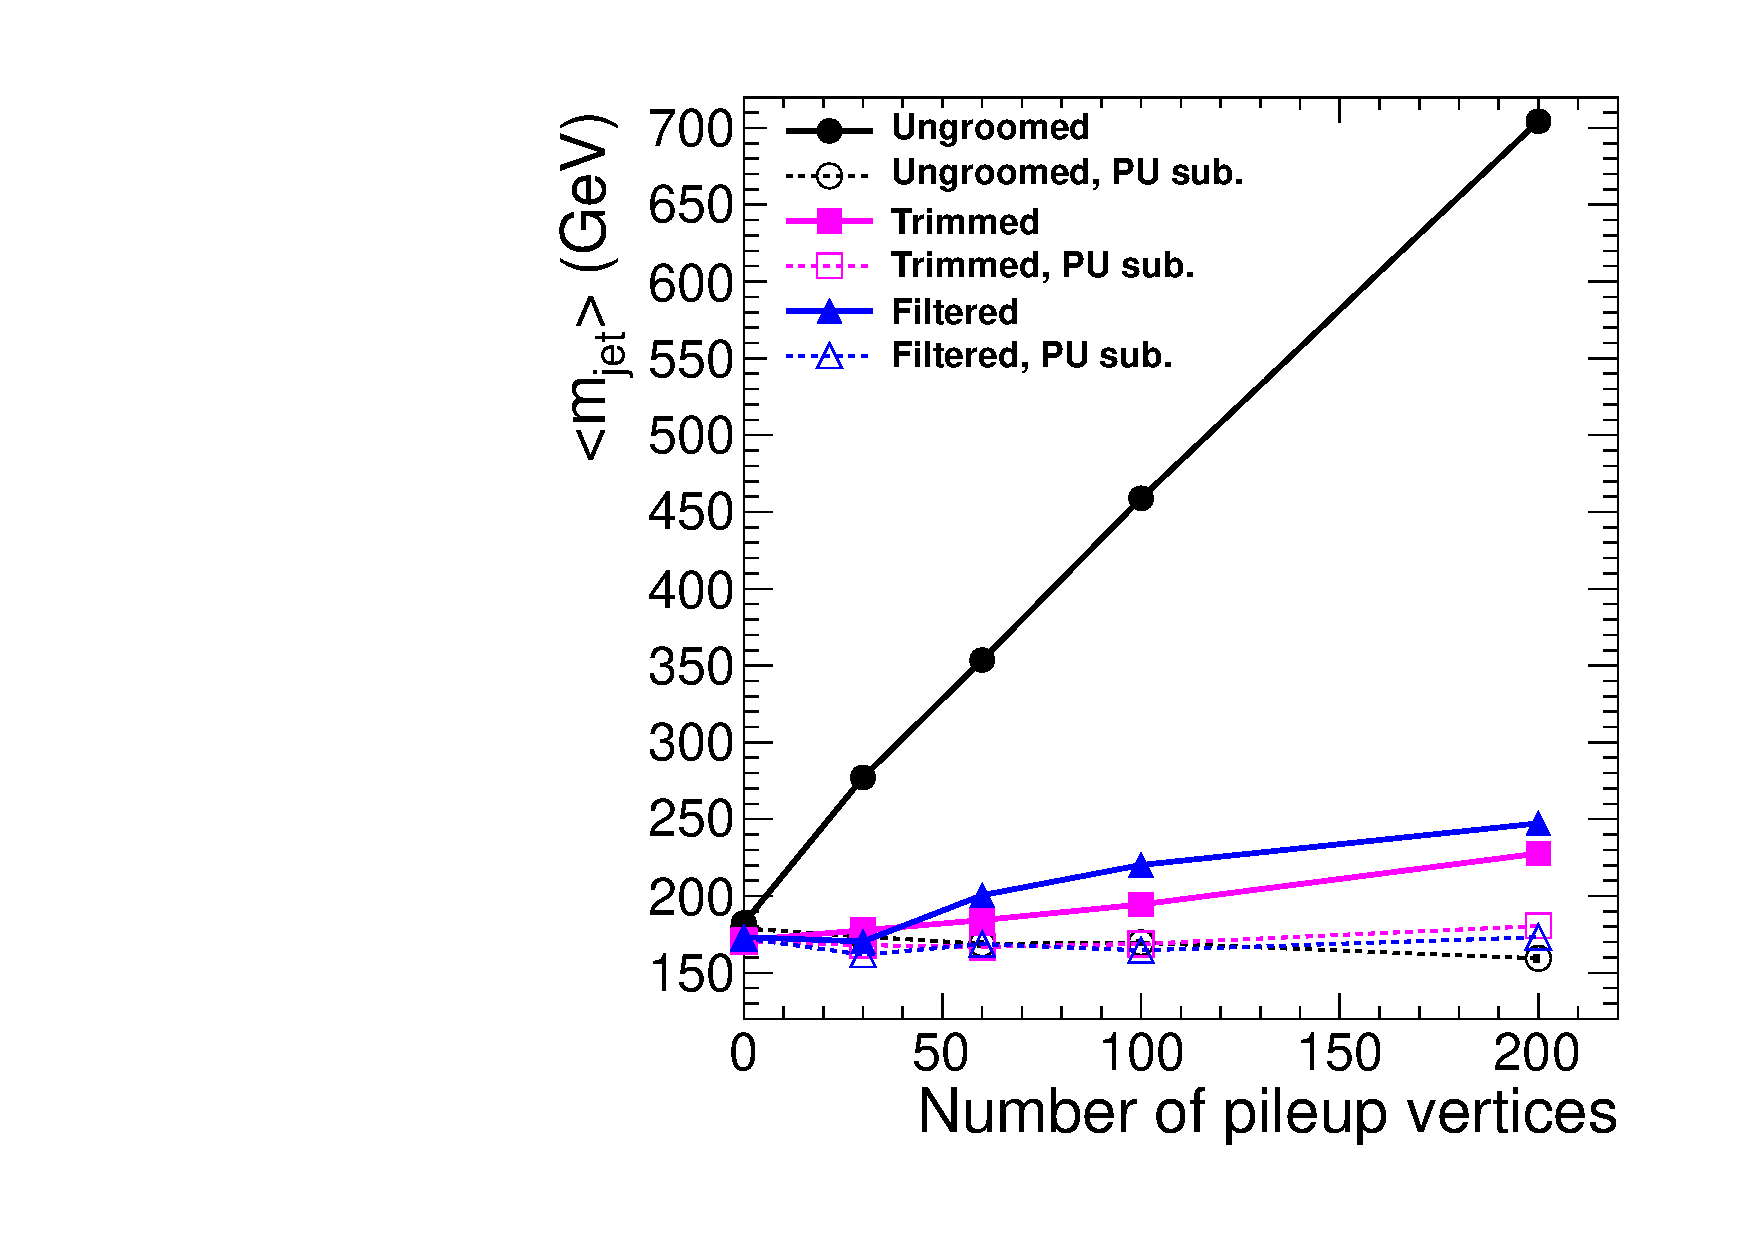
\includegraphics[width=0.45\textwidth]{AK10_mean_vsPU}
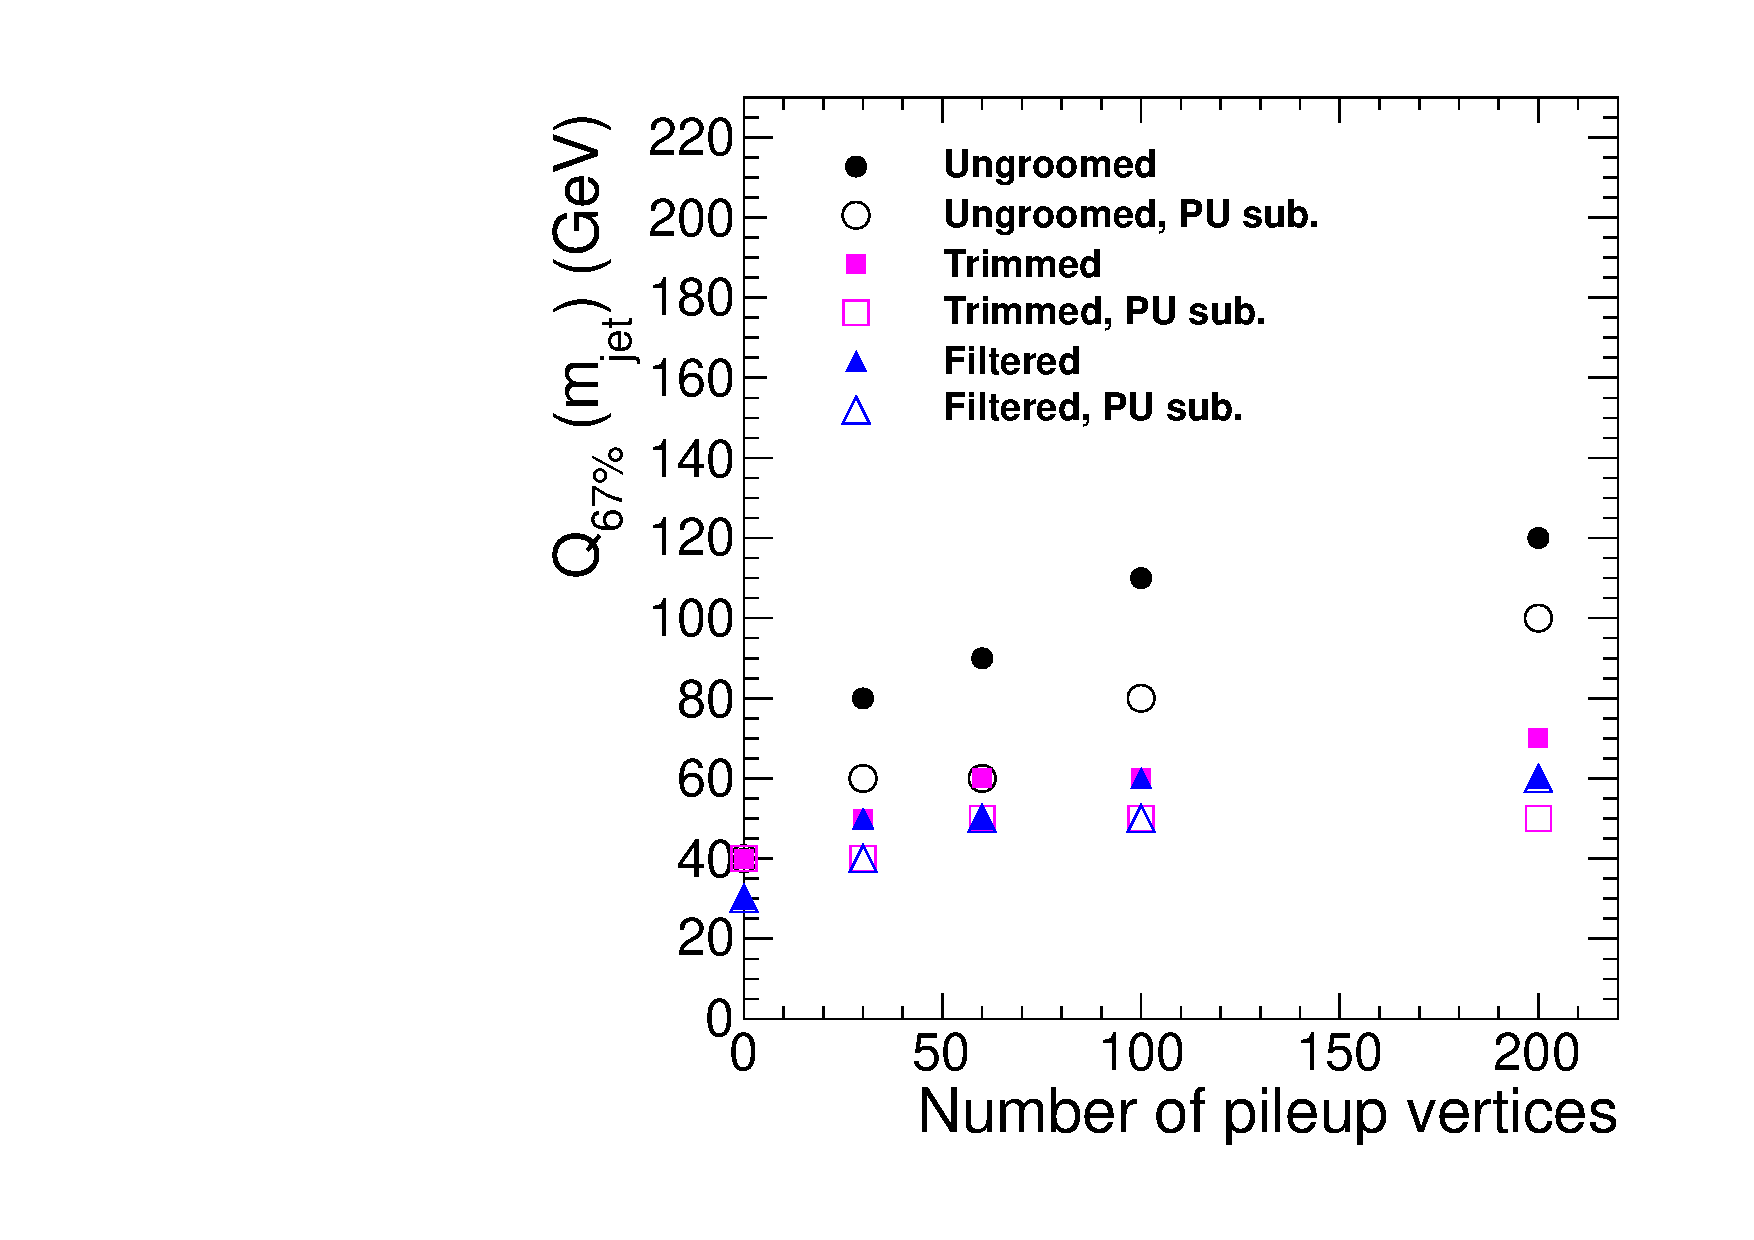
\includegraphics[width=0.45\textwidth]{AK10_rms_vsPU}
\caption[]{Average (leftmost figure) and RMS (rightmost figure) of the reconstructed jet mass distribution in $\Zprime \to \ttbar$ final states, as a function of the pile-up activity \axing, for various jet grooming techniques.}
\label{fig:mass_summary}
\end{center}
\end{figure*}

The findings from the spectra in Figs.~\ref{fig:mass_spectra} are quantitatively summarized in Fig.~\ref{fig:mass_summary} for the mass scale and resolution. Here the resolution is measured in terms of the mass range in which $67\%$ of all jet masses can be found ($Q_{67\%}(m_{\mathrm{jet}})$ quantile).  
Maintaining the jet mass scale around the expectation value of 175~\GeV{} works well for trimming and filtering with and without pile-up subtraction, see Fig.~\ref{fig:mass_summary}. The same figure indicates that for very high pile-up ($\axing = 100 - 200$), the jet mass after trimming and filtering without pile-up subtraction shows increasing sensitivity to the pile-up. The additional pile-up subtraction tends to restore the mass scale with better quality. 



Both trimming and filtering improve the mass resolution to different degrees, but in any case better than pile-up subtraction alone, as expected. Applying the additional pile-up subtraction to trimming yields the least sensitivity to the pile-up activity in terms of mass resolution and scale. 
%
%, while filtering improves the resolution significantly more than those. Applying pile-up subtraction together with trimming and filtering yields the same good mass resolution and scale performance.

%It is also noticeable that pile-up subtraction alone yields a fairly stable jet mass scale, but cannot maintain the mass resolution, as indicated in Fig.~\ref{fig:mass_summary}\subref{fig:mass_summary_rms}. Here filtering with and without pile-up suppression works best. 
%Reconstructing the jet mass after trimming with and without pile-up subtraction yields about the sames resolution performance than just pile-up subtraction. This leads to the conclusion that the manipulation of the jet content  introduced by trimming does not enhance the three prong structure expected from the top-quark decay inside the jet, as the filtering does by keeping only the three hardest sub-jets. 

These effects can be explained as follows. As discussed earlier,
pileup has mainly two effects on the jet: a constant shift
proportional to $\rho A$ and a smearing effect proportional to $\sigma
\sqrt{A}$, with $\sigma$ a measure of the fluctuations of the pileup
within an event. In that language, the subtraction corrects for the
shift leaving the smearing term untouched. Grooming, to the contrary,
since it selects only part of the subjets, acts as if it was reducing
the area of the jet\footnote{Note that grooming techniques do more
  than reducing the catchment area of a jet. Noticeably, the selection
  of the hardest subjets introduces a bias towards including upwards
  fluctuations of the background. This positive bias is balanced by a
  negative one related to the perturbative radiation discarded by the
  grooming. These effects go beyond the generic features explained
  here.}. This reduces both the shift and the dispersion. Combining
grooming with subtraction thus allows to correct for the shift
leftover by grooming and reduce the smearing effects at the same
time. All these effects are observed in Figures~\ref{fig:mass_summary}.
  



%From the plots in Fig.~\ref{fig:mass_summary} it is obvious that in this exercise pruning does not help with maintaining the mass scale and resolution in the presence of pile-up. Even when applying the pile-up subtraction in addition, the mass scale of the pruned jet still shows a significant dependence on \axing{} (see Fig.~\ref{fig:mass_summary}\subref{fig:mass_summary_ave}), and the resolution performance is not improved with respect to just the pile-up subtraction by itself (see Fig.~\ref{fig:mass_summary}\subref{fig:mass_summary_rms}).   

\subsection{Concluding remarks}\label{subsec:concl}

The source of jets produced in minimum bias collisions in the presence of \pu{} is analyzed using a technique relating the single collision contribution in the jet to its transverse momentum after \pu{} correction in particle level Monte Carlo. The rate of \pujet s surviving after application of the jet area based \pu{} subtraction is about two with $\ptcorr > 20$~\GeV{} and within $|y|<2$, at a \pu{} activity of $\axing = 100$. It rises about linearly with increasing pile-up for this particular selection. Higher \pT{} jets occur at a much reduced rate, but with a steeper than linear rise with increasing $\mu$. 

The rate of QCD-like jets is significantly smaller, and shows a less-than-linear increase with increasing $\mu$ even for $\pTmin = 20$~\GeV. This can be understood as a sign of increased merging between QCD-like jets and stochastic jets. The merged jets are less likely to display features characteristic for QCD-like jets, and therefore fail the selection. 

The fraction of QCD-like jets with a core of energy arising from a single \pp{} interaction of at least $0.8 \ptcorr$ is found to decrease rapidly with
increasing $\mu$. At $\mu=50$ about 60\% of the \pu{} jets with $\ptcorr > 50\GeV$ are found to be QCD-like, whereas at $\mu=200$ this number is decreased to 
about 20\%.



A brief Monte Carlo study of the effect of jet grooming techniques on
the jet mass reconstruction in $\Zprime \to \ttbar$ final states has
been conducted. Jet trimming and filtering are used by themselves, or
in combination with the pile-up subtraction using the four-vector
area, to reconstruct the single jet mass and evaluate the stability of
the mass scale and resolution at pile-up levels of 30, 60, 100, and
200 extra \pp{} collisions, in addition to the signal event. It is
found that for this particular final state trimming and filtering work
well for maintaining the mass scale and resolution, provided they are
applied together with pile-up subtraction so as to benefit both from
the average shift correction from subtraction and noise reduction from
the grooming. 
% especially when applied together with overall pile-up subtraction. 
%
%Trimming  yields comparable results for the mass scale, but does not restore the resolution as well. 
%Jet pruning is the least performing technique with respect to pile-up suppression. In general the observations in this study support the notion that a grooming tool like the filtering configuration used here, which is geared to extract the three prong decay structure of the top-quarks, perform better than the techniques based on the removal of diffuse contributions without a goal of extracting a specific decay structure.

The studies presented here are performed with Monte Carlo simulated signal and pile-up (minimum bias) interactions. No considerations have been given to detector sensitivities and other effects deteriorating the stable particle level kinematics and flows exploited here. With this respect the conclusions of this study are limited and can be considered optimistic until shown otherwise.     
%
Note also that comparing the performance of filtering and trimming
would require varying their parameters and that this goes beyond the
scope of this study.


%\bibliographystyle{boostnote}
%\bibliography{boostbib}

%\end{document}
